\newcommand{\shapefigurepartbase}[4]{
  \begin{subfigure}{0.2\textwidth}
    \includegraphics[width=\linewidth]{assets/images/shapes/#2/#1#3}
    \caption{\makefirstuc{#2 #4}}
    \label{fig:#2_#1#3}
  \end{subfigure}
}

\newcommand{\shapefigurepart}[2]{
  \shapefigurepartbase{#1}{#2}{}{model}
}

\newcommand{\shapefigurepartw}[2]{
  \shapefigurepartbase{#1}{#2}{_w}{wireframe}
}

\newcommand{\shapefigure}[2]{
\begin{figure}
  \begin{center}
    \shapefigurepart{#1}{old}
    \shapefigurepartw{#1}{old}
    \shapefigurepart{#1}{new}
    \shapefigurepartw{#1}{new}
  \end{center}
  \caption{\makefirstuc{#2 molecule mesh implementation.}}
  \label{fig:#1_shape}
\end{figure}
}

\newcommand{\oldshapefigure}[1]{
\begin{figure}
  \begin{center}
    \shapefigurepart{#1}{old}
    \shapefigurepartw{#1}{old}
  \end{center}
  \caption{\makefirstuc{#1}}
  \label{fig:#1_shape}
\end{figure}
}

\newcommand{\newshapefigure}[2]{
\begin{figure}
  \begin{center}
    \shapefigurepart{#1}{new}
    \shapefigurepartw{#1}{new}
  \end{center}
  \caption{\makefirstuc{#2}}
  \label{fig:#1_shape}
\end{figure}
}

\section{Shapes}
\subsection{WebMGA 2.0 Implementation}
WebMGA 2.0 implements the following molecule shapes:
\begin{itemize}
  \item Sphere (\cref{fig:sphere_shape})
  \item Ellipsoid (\cref{fig:ellipsoid_shape})
  \item Spherocylinder (\cref{fig:spherocylinder_shape})
  \item Spheroplatelet (\cref{fig:spheroplatelet_shape})
  \item Cut Sphere (\cref{fig:doublecutsphere_shape}, implemented as a double cut sphere)
  \item Cylinder (\cref{fig:cylinder_shape})
  \item Torus (\cref{fig:torus_shape})
\end{itemize}
Notably missing but useful are the single cut sphere, the spherical cap, and the lens. The cylinder and torus shapes are present since the three.js library provides easily callable predefined meshes, however serve little practical purpose since no realistic molecular configuration would model using these.
\oldshapefigure{cylinder}
\oldshapefigure{torus}

\subsection{WebMGA 2.0 Bugs}
\begin{figure}
  \begin{center}
    \begin{subfigure}{0.2\textwidth}
    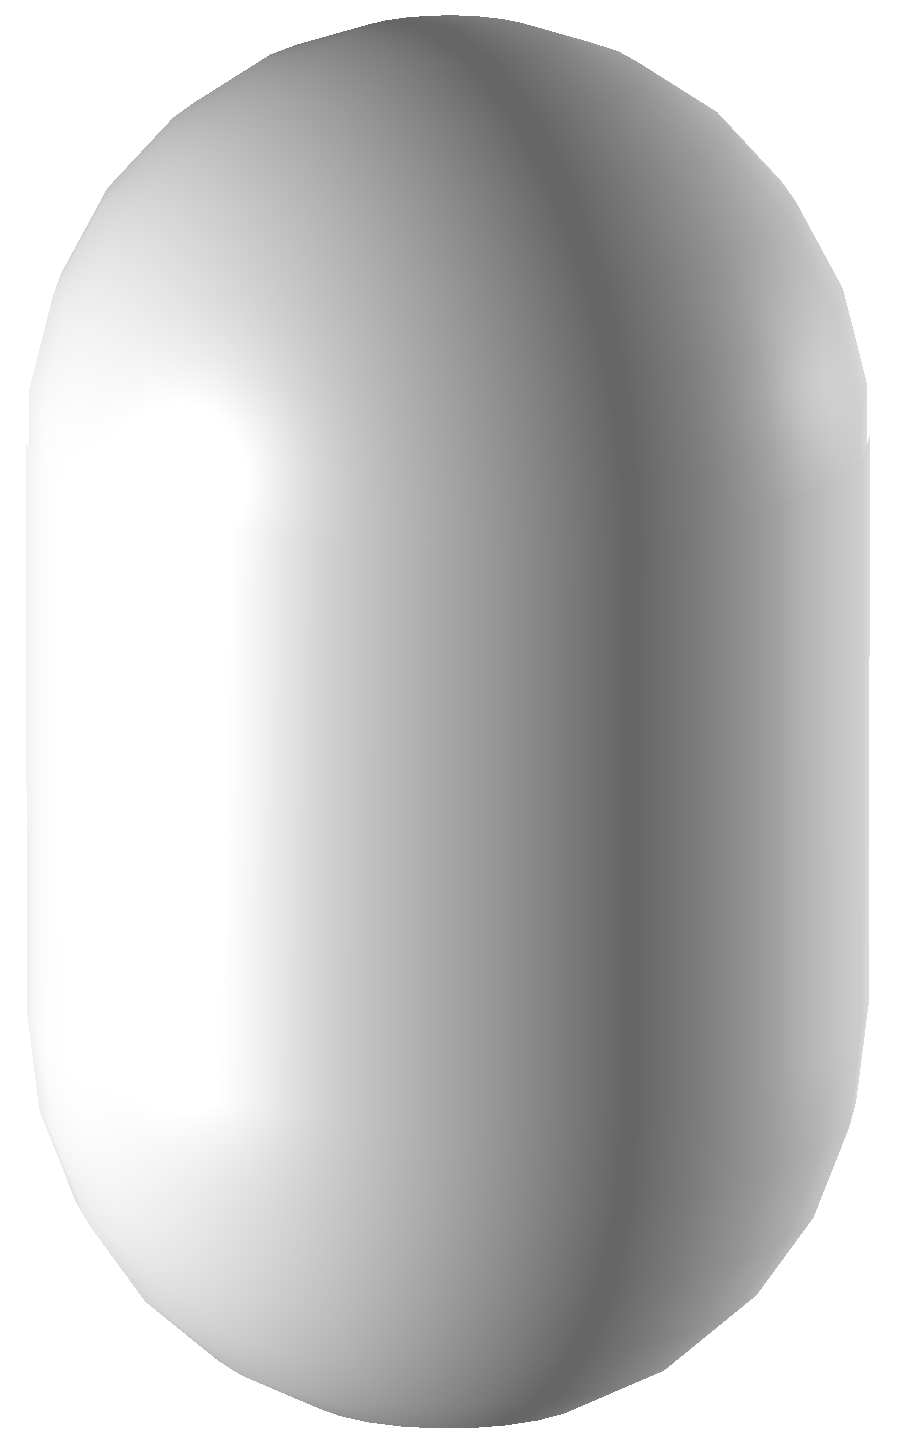
\includegraphics[width=\linewidth]{assets/images/shapes/bugold/bad_mesh_high}
    \caption{\makefirstuc{WebMGA 2.0 high detail shape}}
    \end{subfigure}
      \begin{subfigure}{0.2\textwidth}
    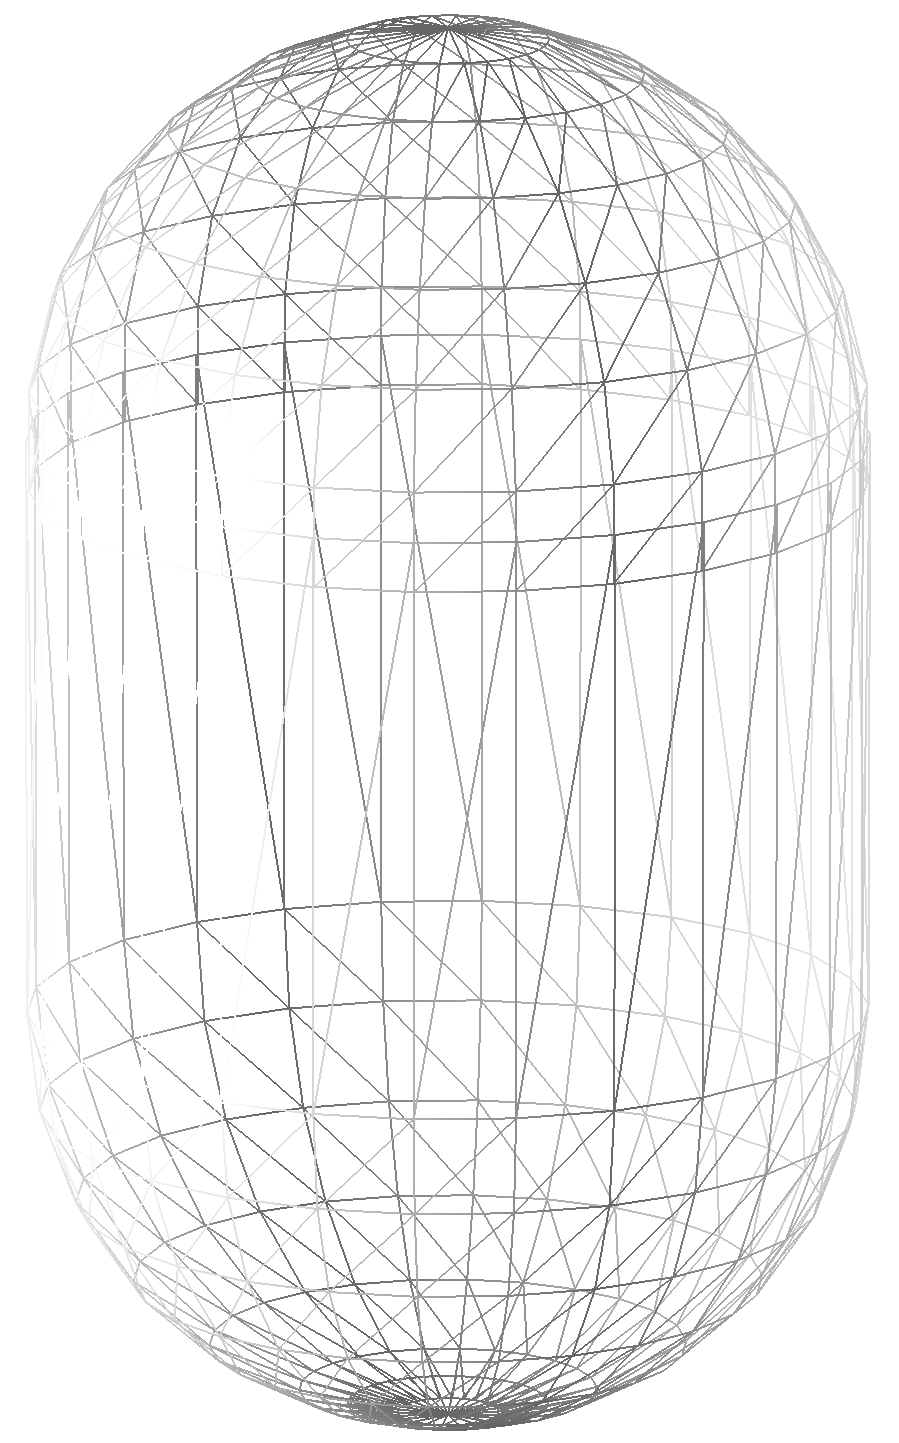
\includegraphics[width=\linewidth]{assets/images/shapes/bugold/bad_mesh_high_w}
    \caption{\makefirstuc{WebMGA 2.0 high detail mesh}}
    \end{subfigure}
    \begin{subfigure}{0.2\textwidth}
    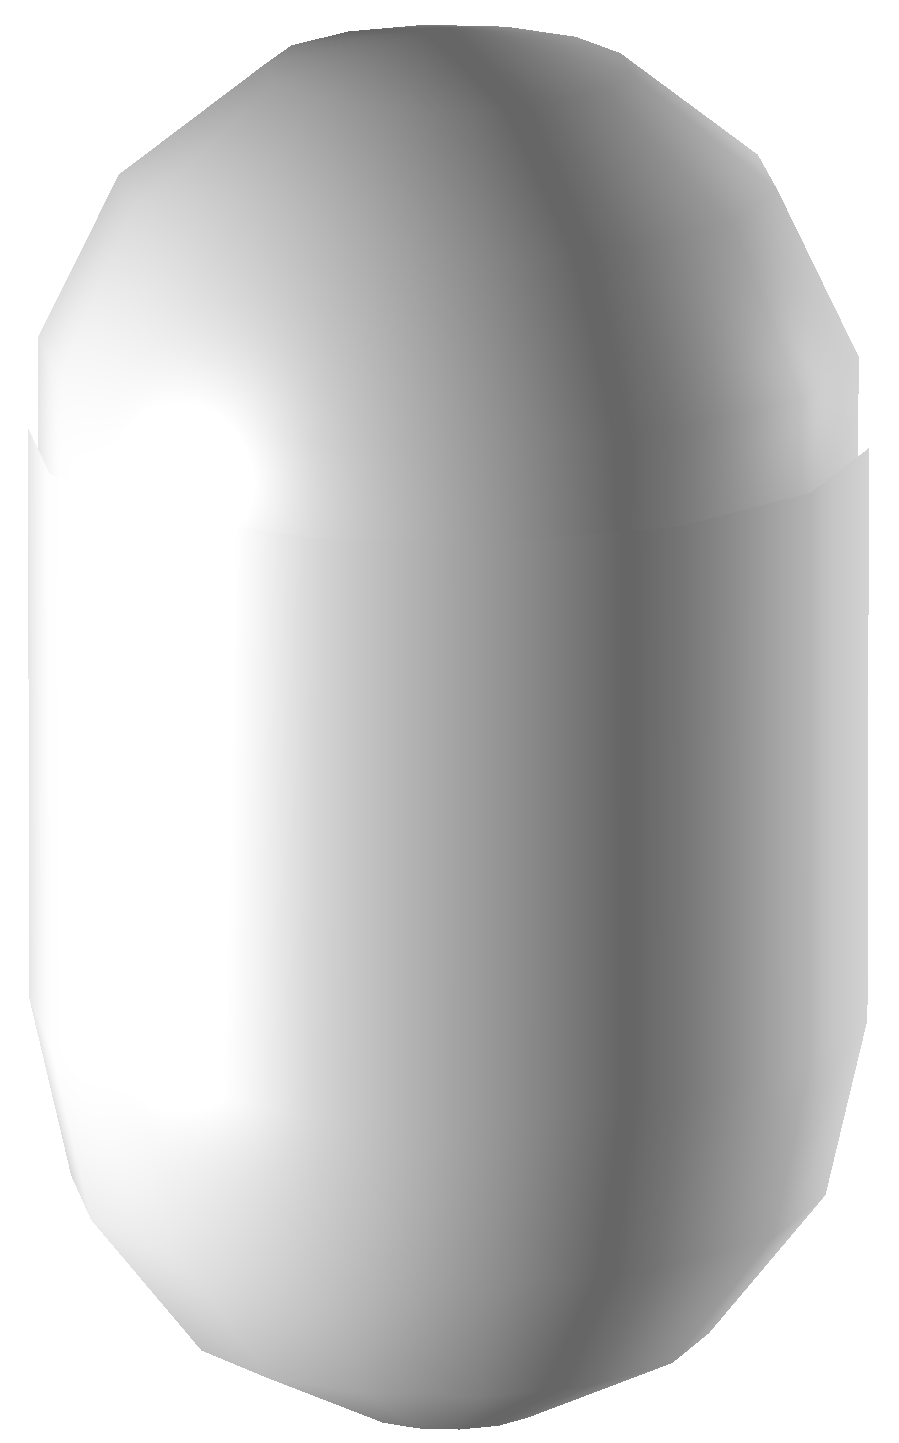
\includegraphics[width=\linewidth]{assets/images/shapes/bugold/bad_mesh_med}
    \caption{\makefirstuc{WebMGA 2.0 medium detail shape}}
    \end{subfigure}
    \begin{subfigure}{0.2\textwidth}
    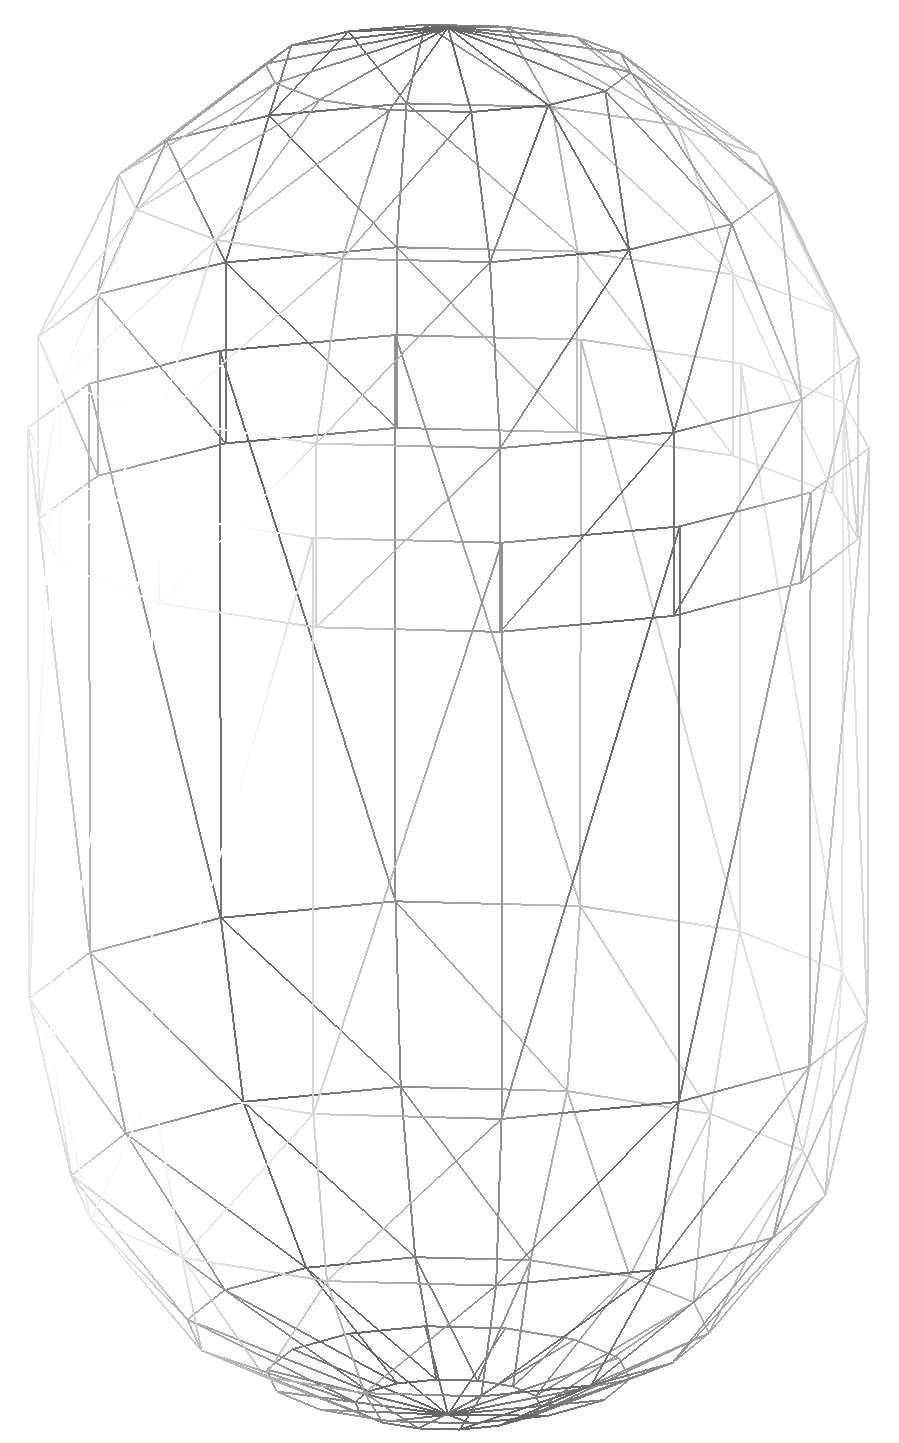
\includegraphics[width=\linewidth]{assets/images/shapes/bugold/bad_mesh_med_w}
    \caption{\makefirstuc{WebMGA 2.0 medium detail mesh}}
    \end{subfigure}
    \begin{subfigure}{0.2\textwidth}
    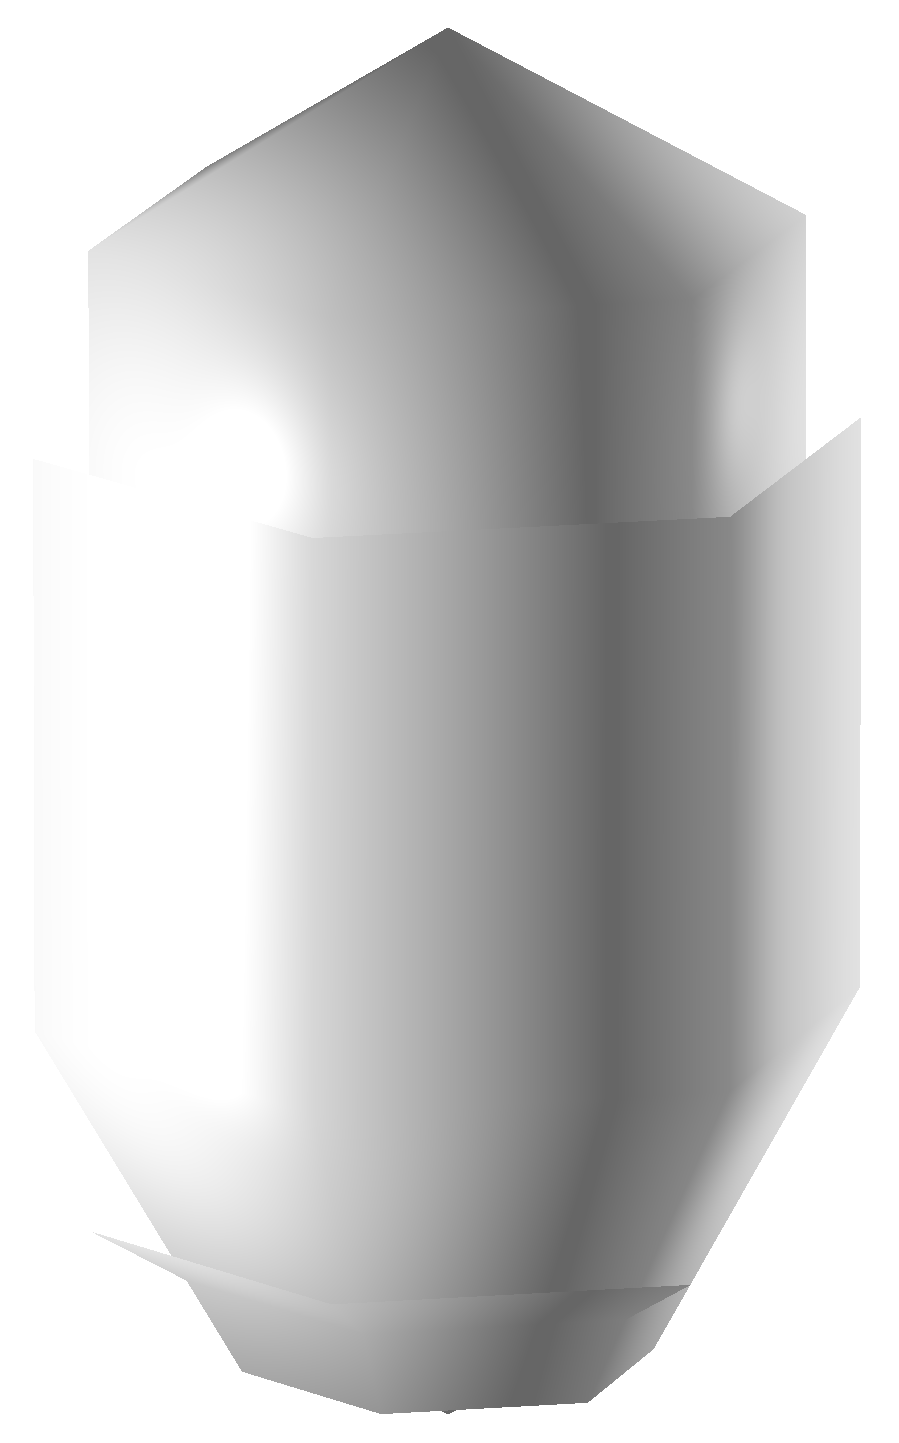
\includegraphics[width=\linewidth]{assets/images/shapes/bugold/bad_mesh_low}
    \caption{\makefirstuc{WebMGA 2.0 low detail shape}}
    \end{subfigure}
    \begin{subfigure}{0.2\textwidth}
    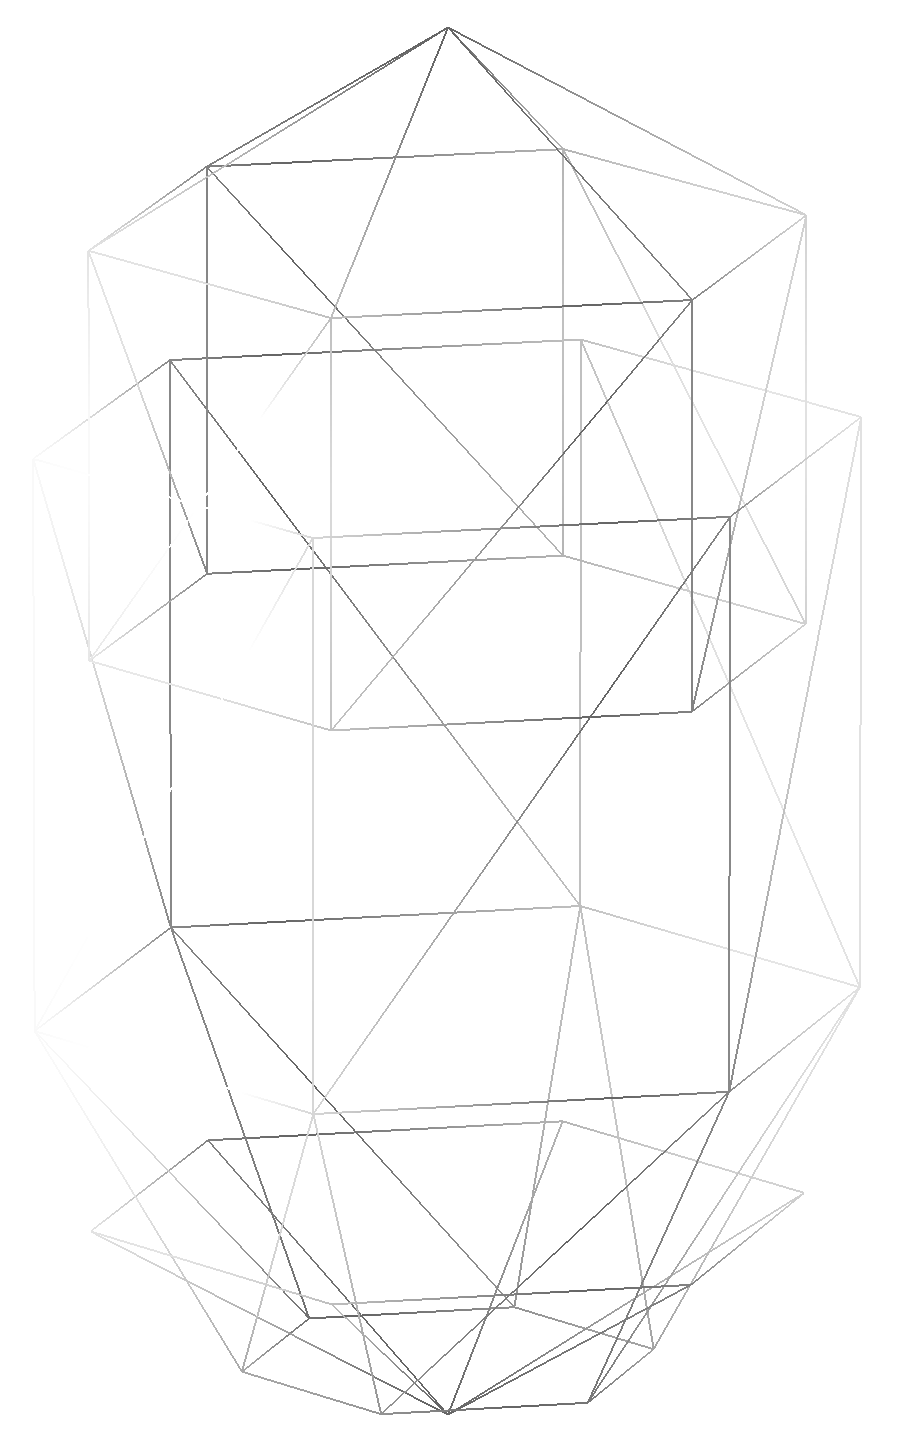
\includegraphics[width=\linewidth]{assets/images/shapes/bugold/bad_mesh_low_w}
    \caption{\makefirstuc{WebMGA 2.0 low detail mesh}}
    \end{subfigure}
  \end{center}
  \caption{\makefirstuc{Bad spheocylinder mesh generated by WebMGA 2.0}}
  \label{fig:bad_spherocylinder_old}
\end{figure}
\begin{figure}
  \begin{center}
    \begin{subfigure}{0.2\textwidth}
    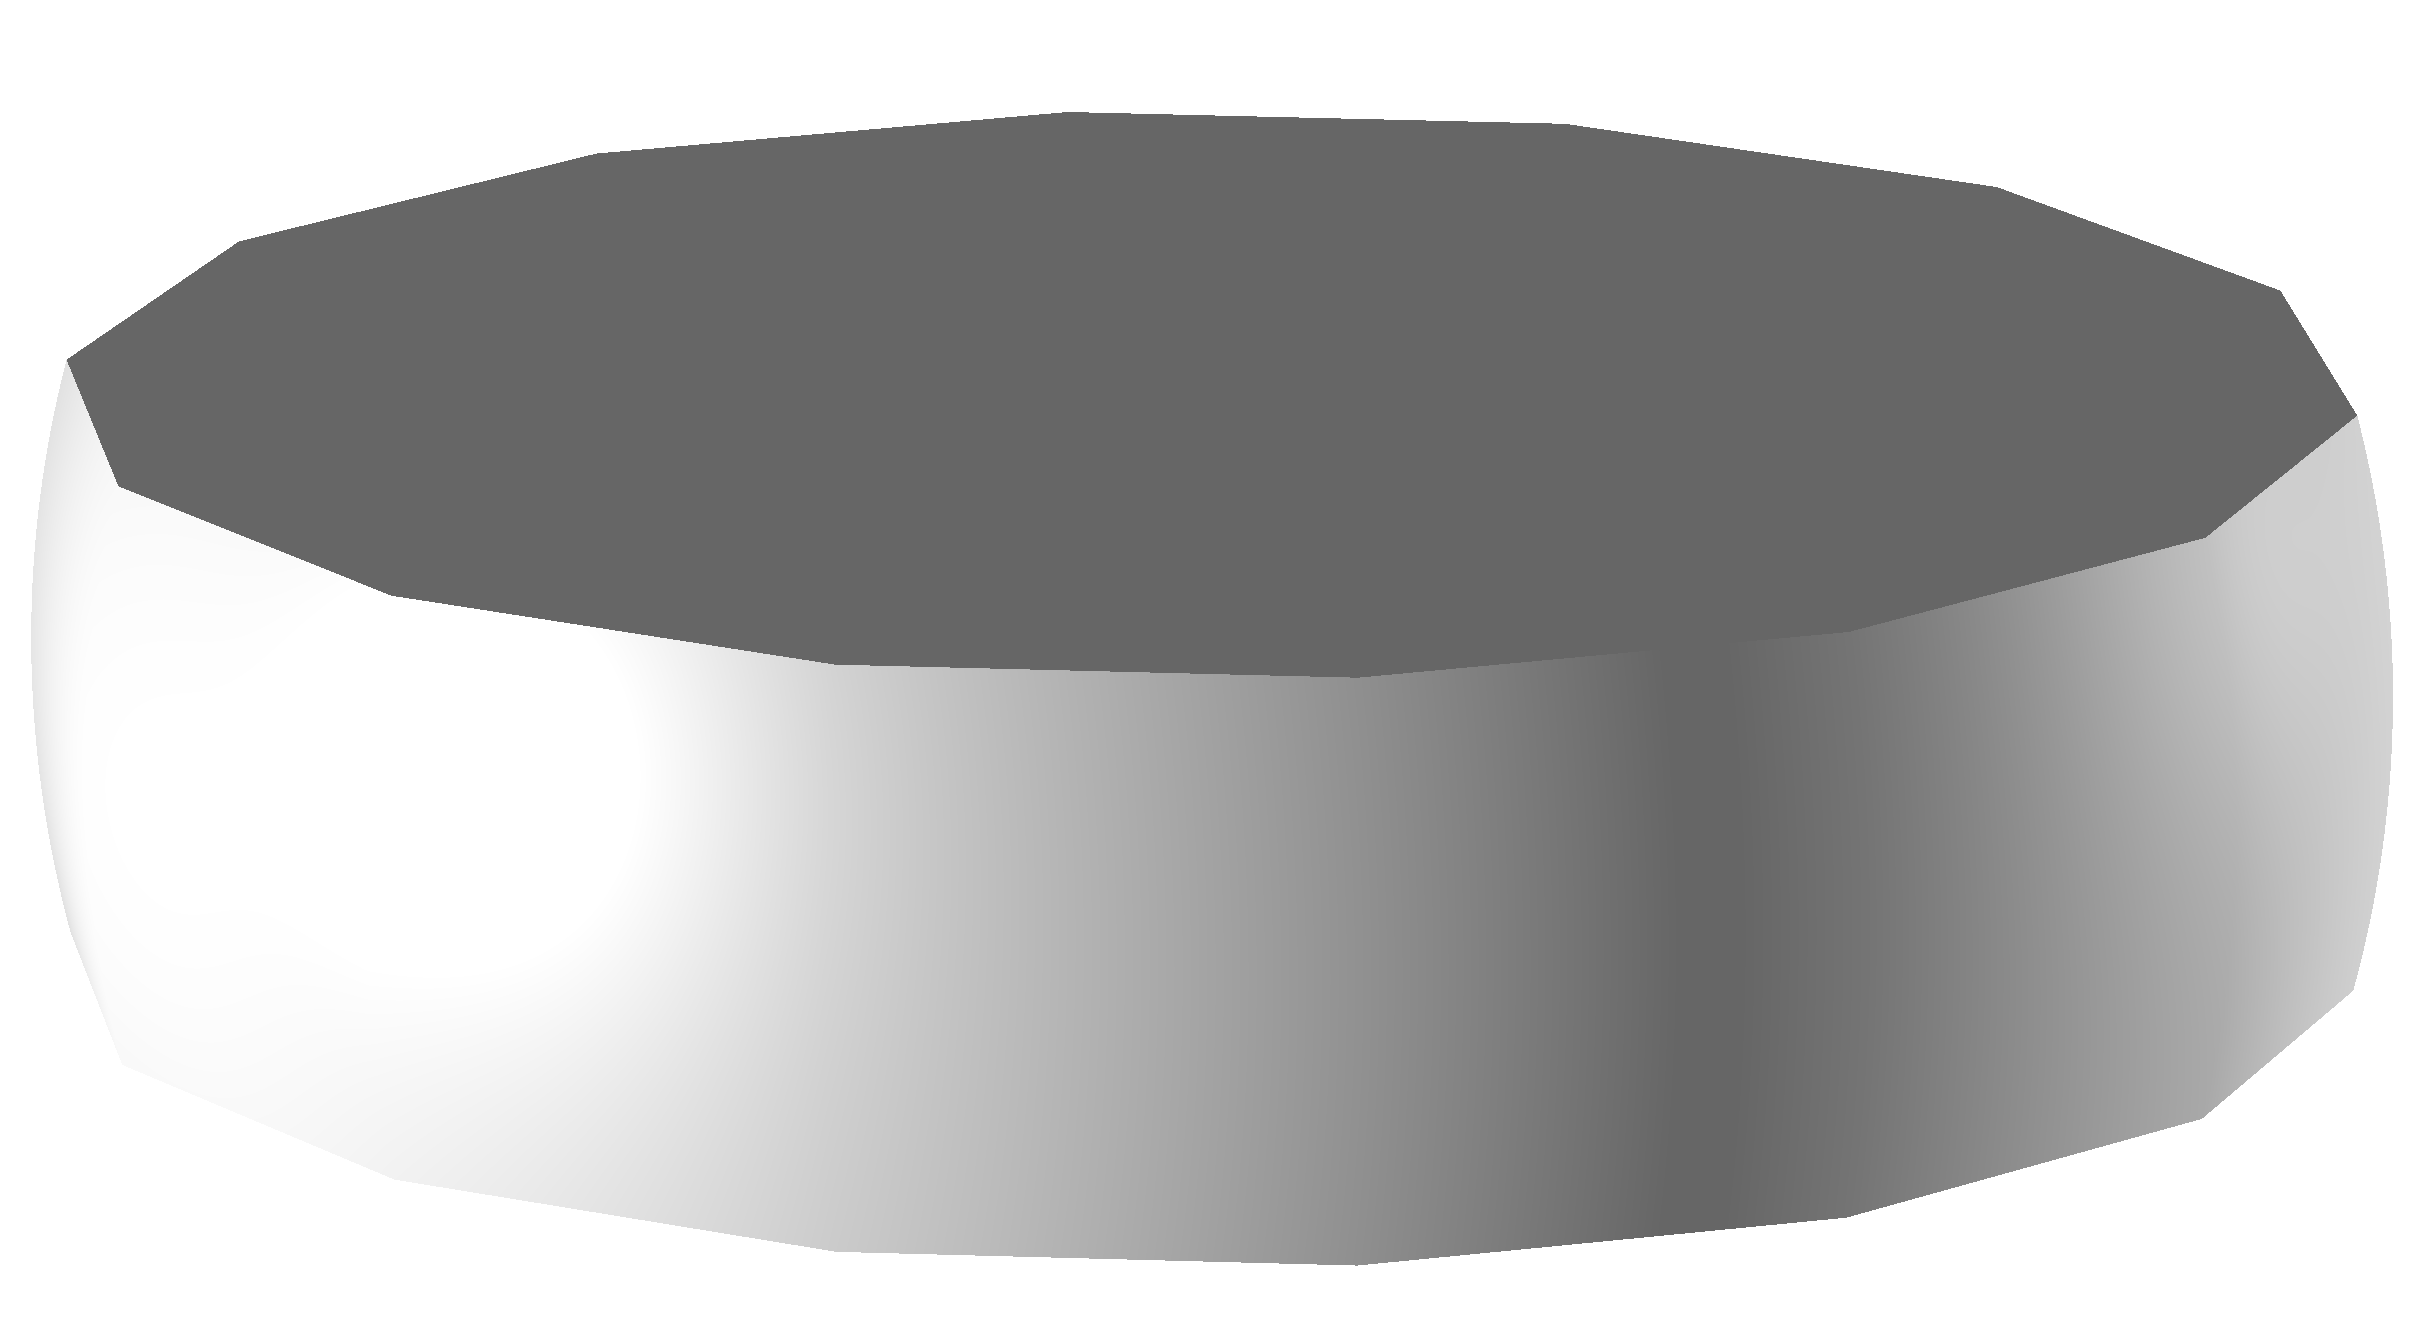
\includegraphics[width=\linewidth]{assets/images/shapes/bugold/scale_high}
    \caption{\makefirstuc{WebMGA 2.0}}
    \end{subfigure}
      \begin{subfigure}{0.2\textwidth}
    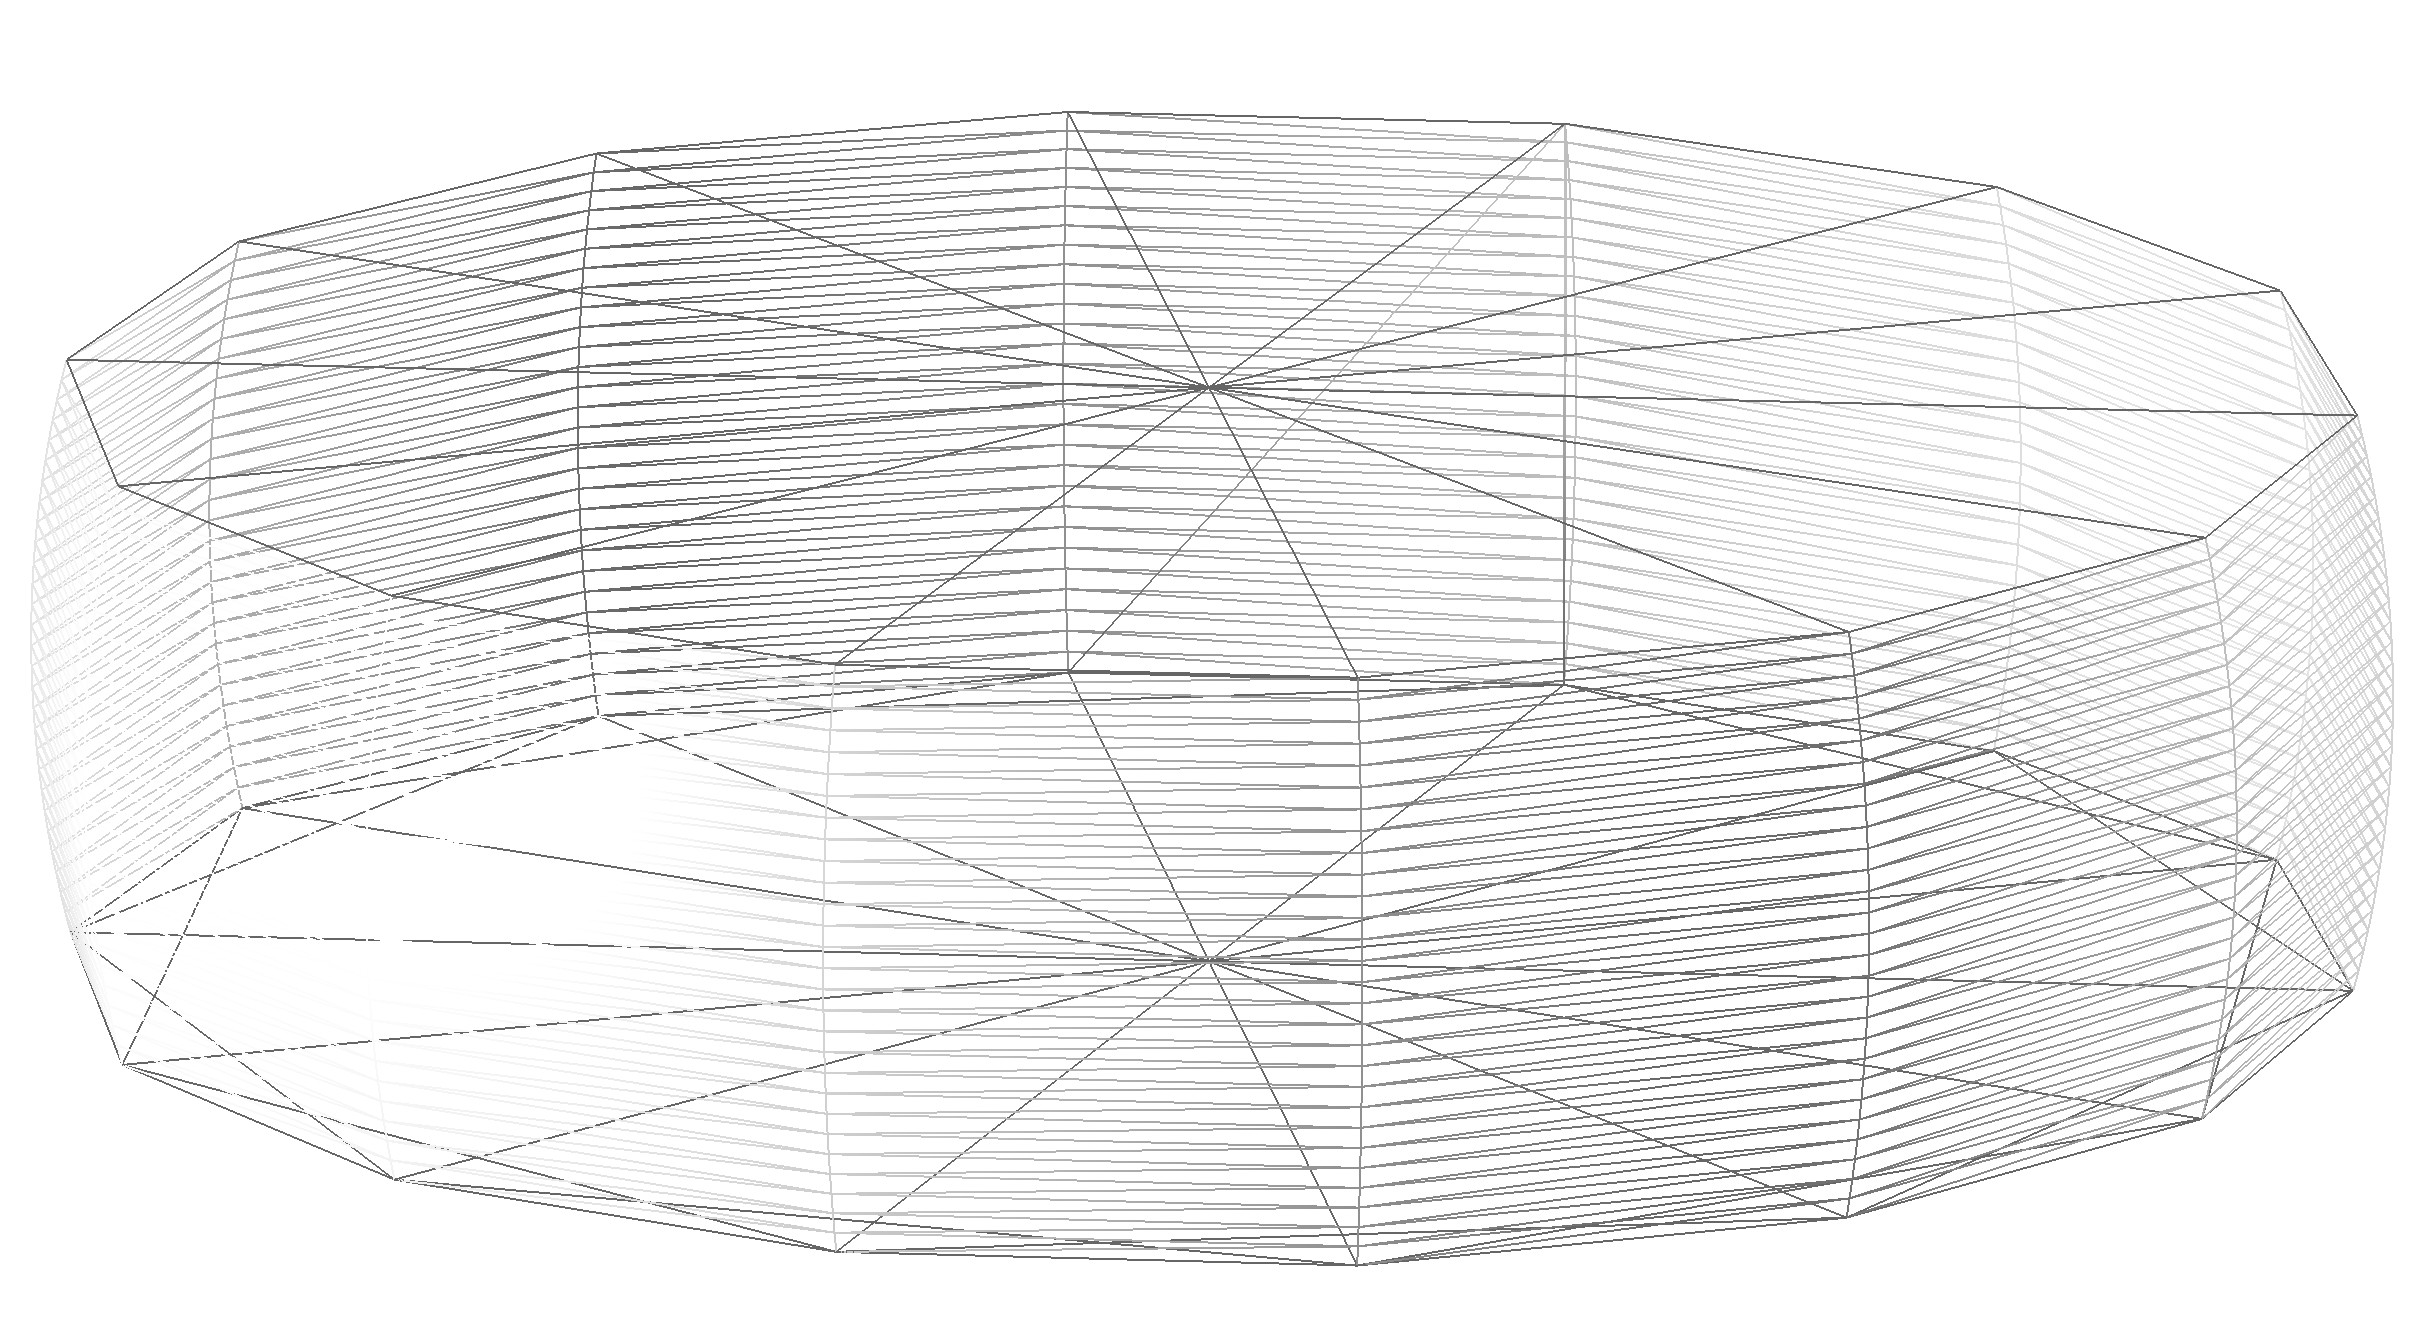
\includegraphics[width=\linewidth]{assets/images/shapes/bugold/scale_high_w}
    \caption{\makefirstuc{WebMGA 2.0}}
    \end{subfigure}
    \begin{subfigure}{0.2\textwidth}
    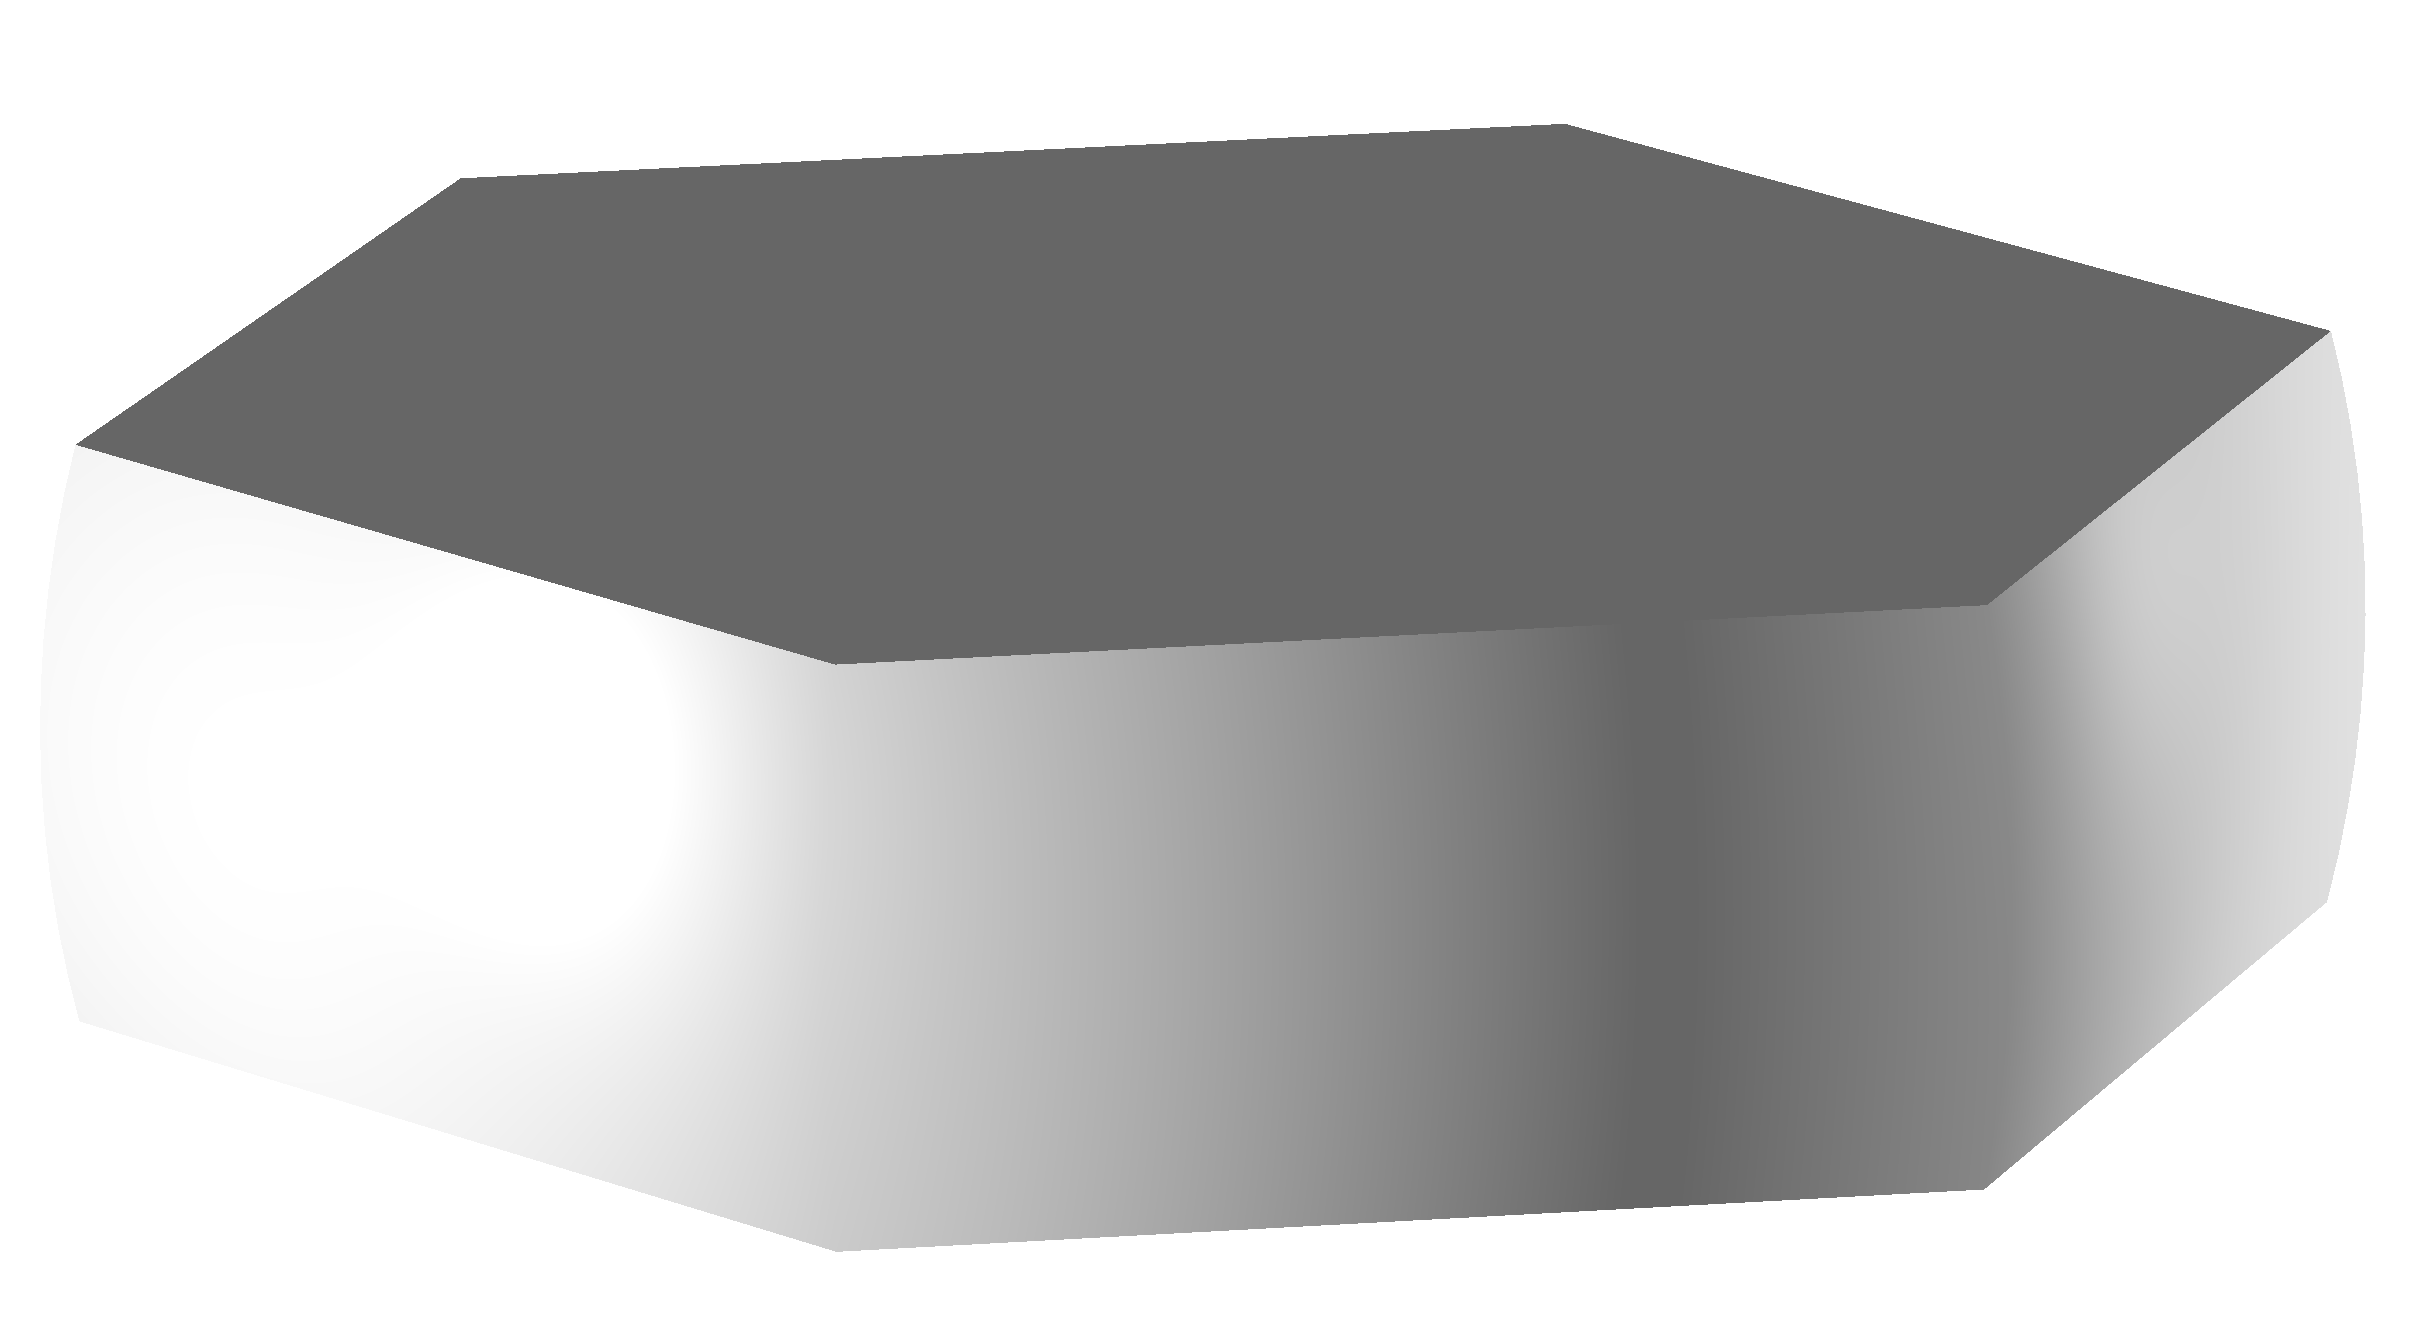
\includegraphics[width=\linewidth]{assets/images/shapes/bugold/scale_low}
    \caption{\makefirstuc{WebMGA 2.0}}
    \end{subfigure}
    \begin{subfigure}{0.2\textwidth}
    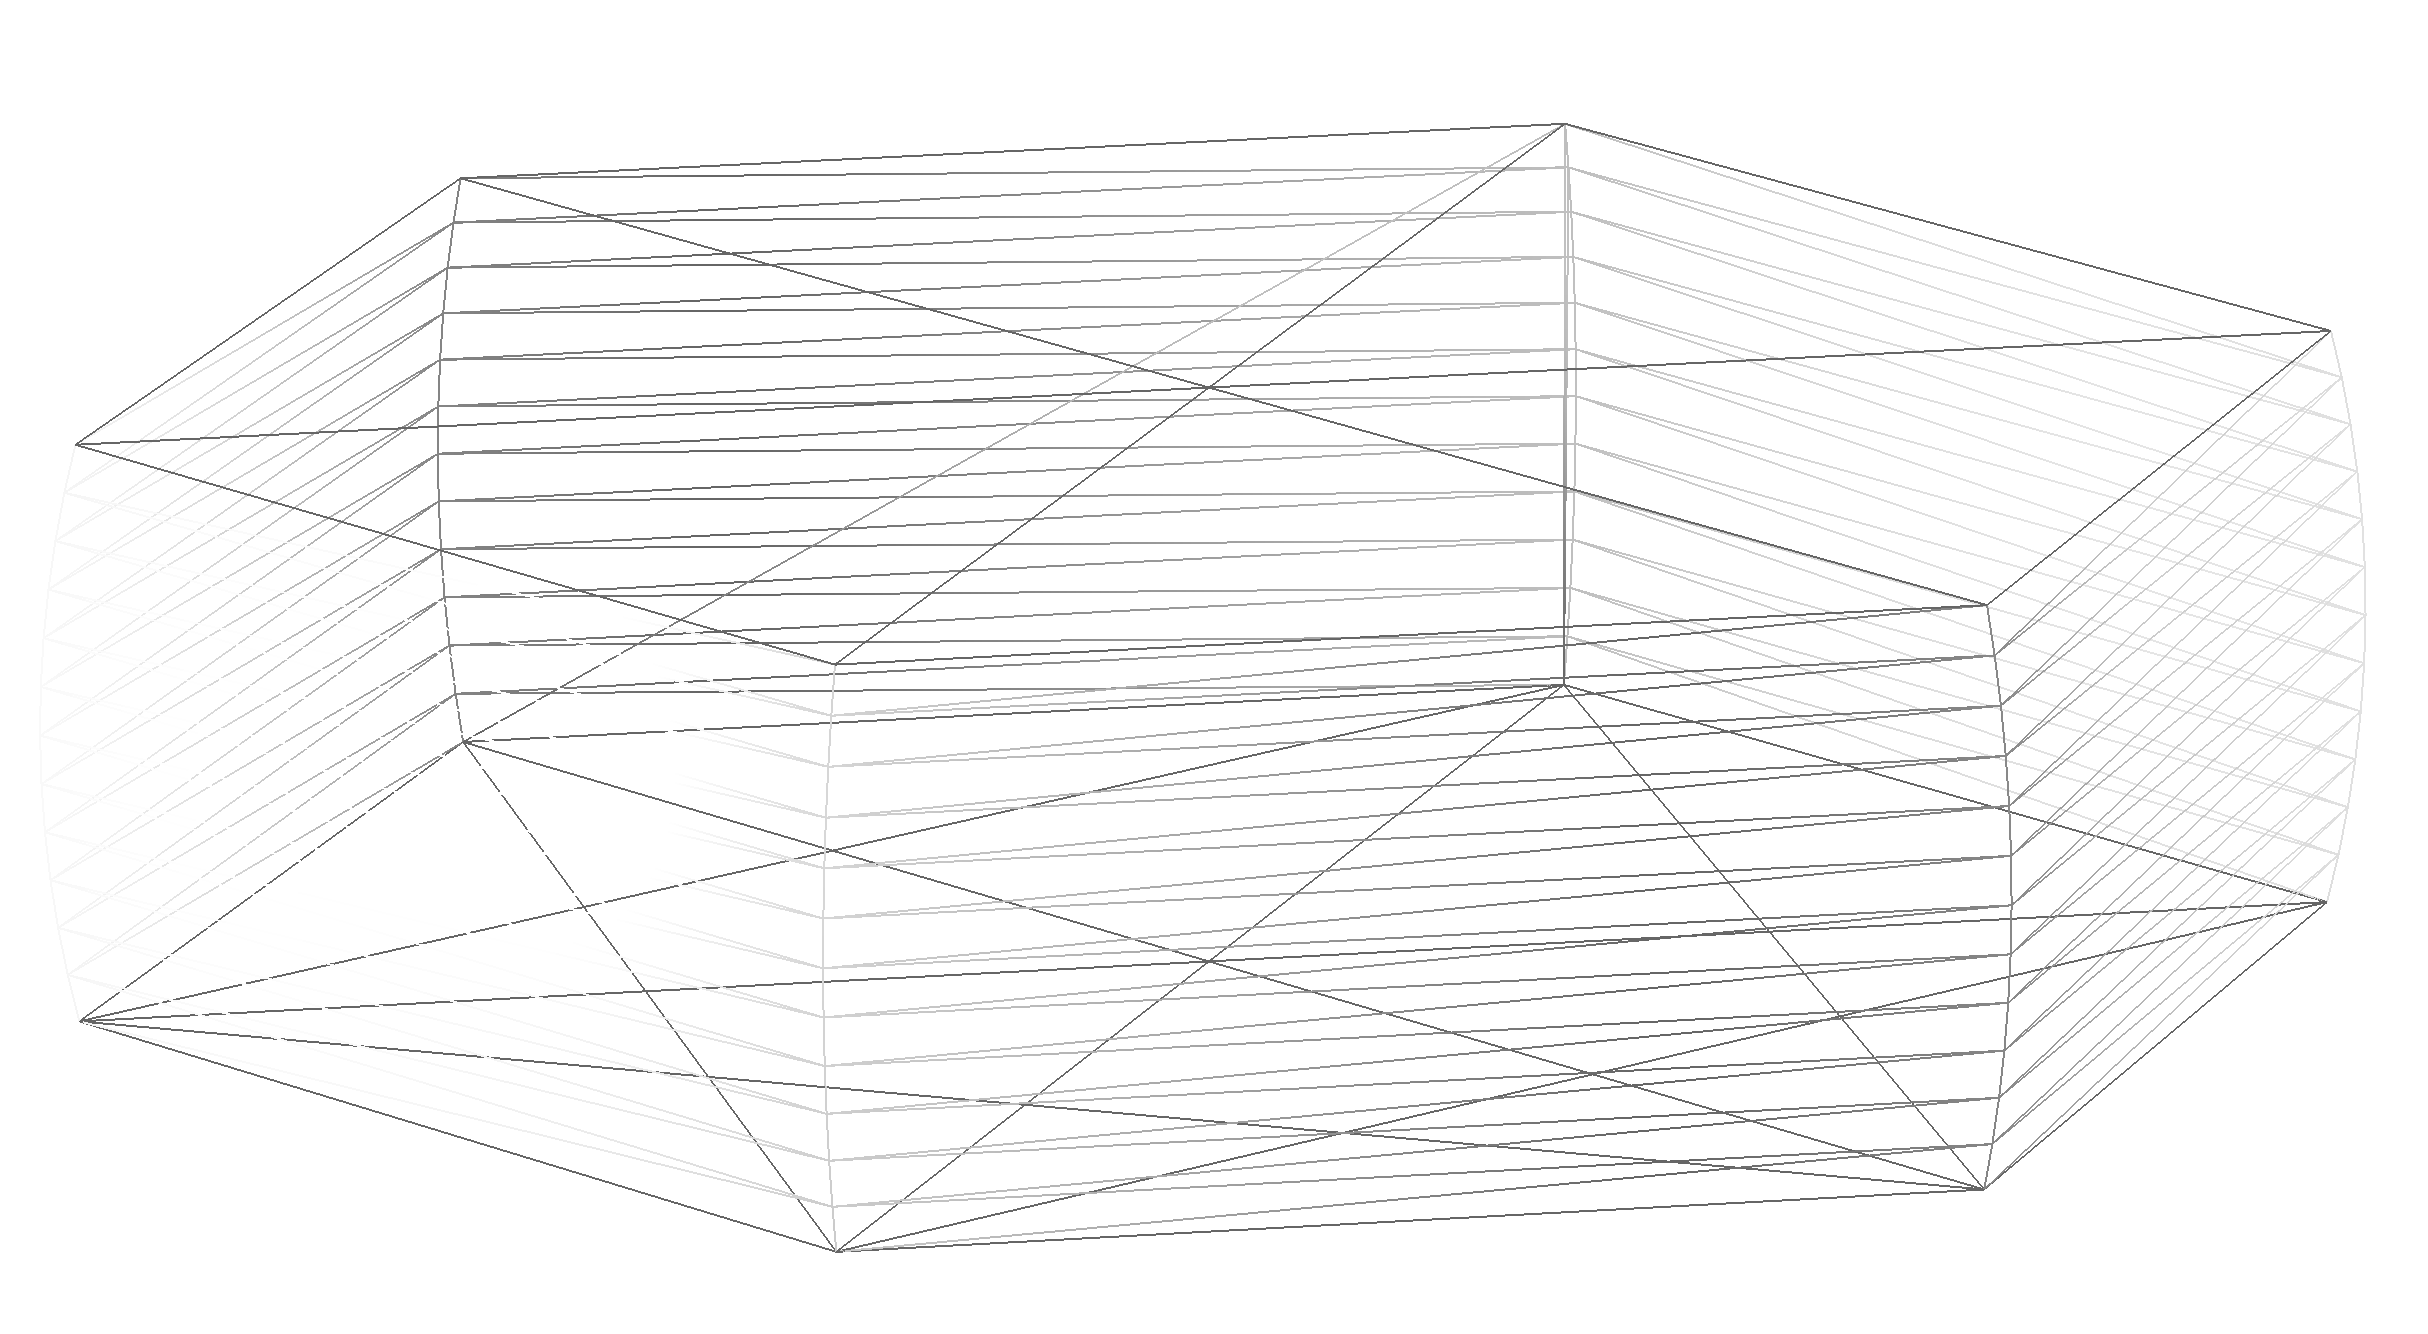
\includegraphics[width=\linewidth]{assets/images/shapes/bugold/scale_low_w}
    \caption{\makefirstuc{WebMGA 2.0}}
    \end{subfigure}
  \end{center}
  \caption{\makefirstuc{Notably higher mesh quality vertically for double cut sphere with WebMGA 2.0}}
  \label{fig:uneven_mesh_old}
\end{figure}
\begin{figure}
  \begin{center}
    \begin{subfigure}{0.4\textwidth}
    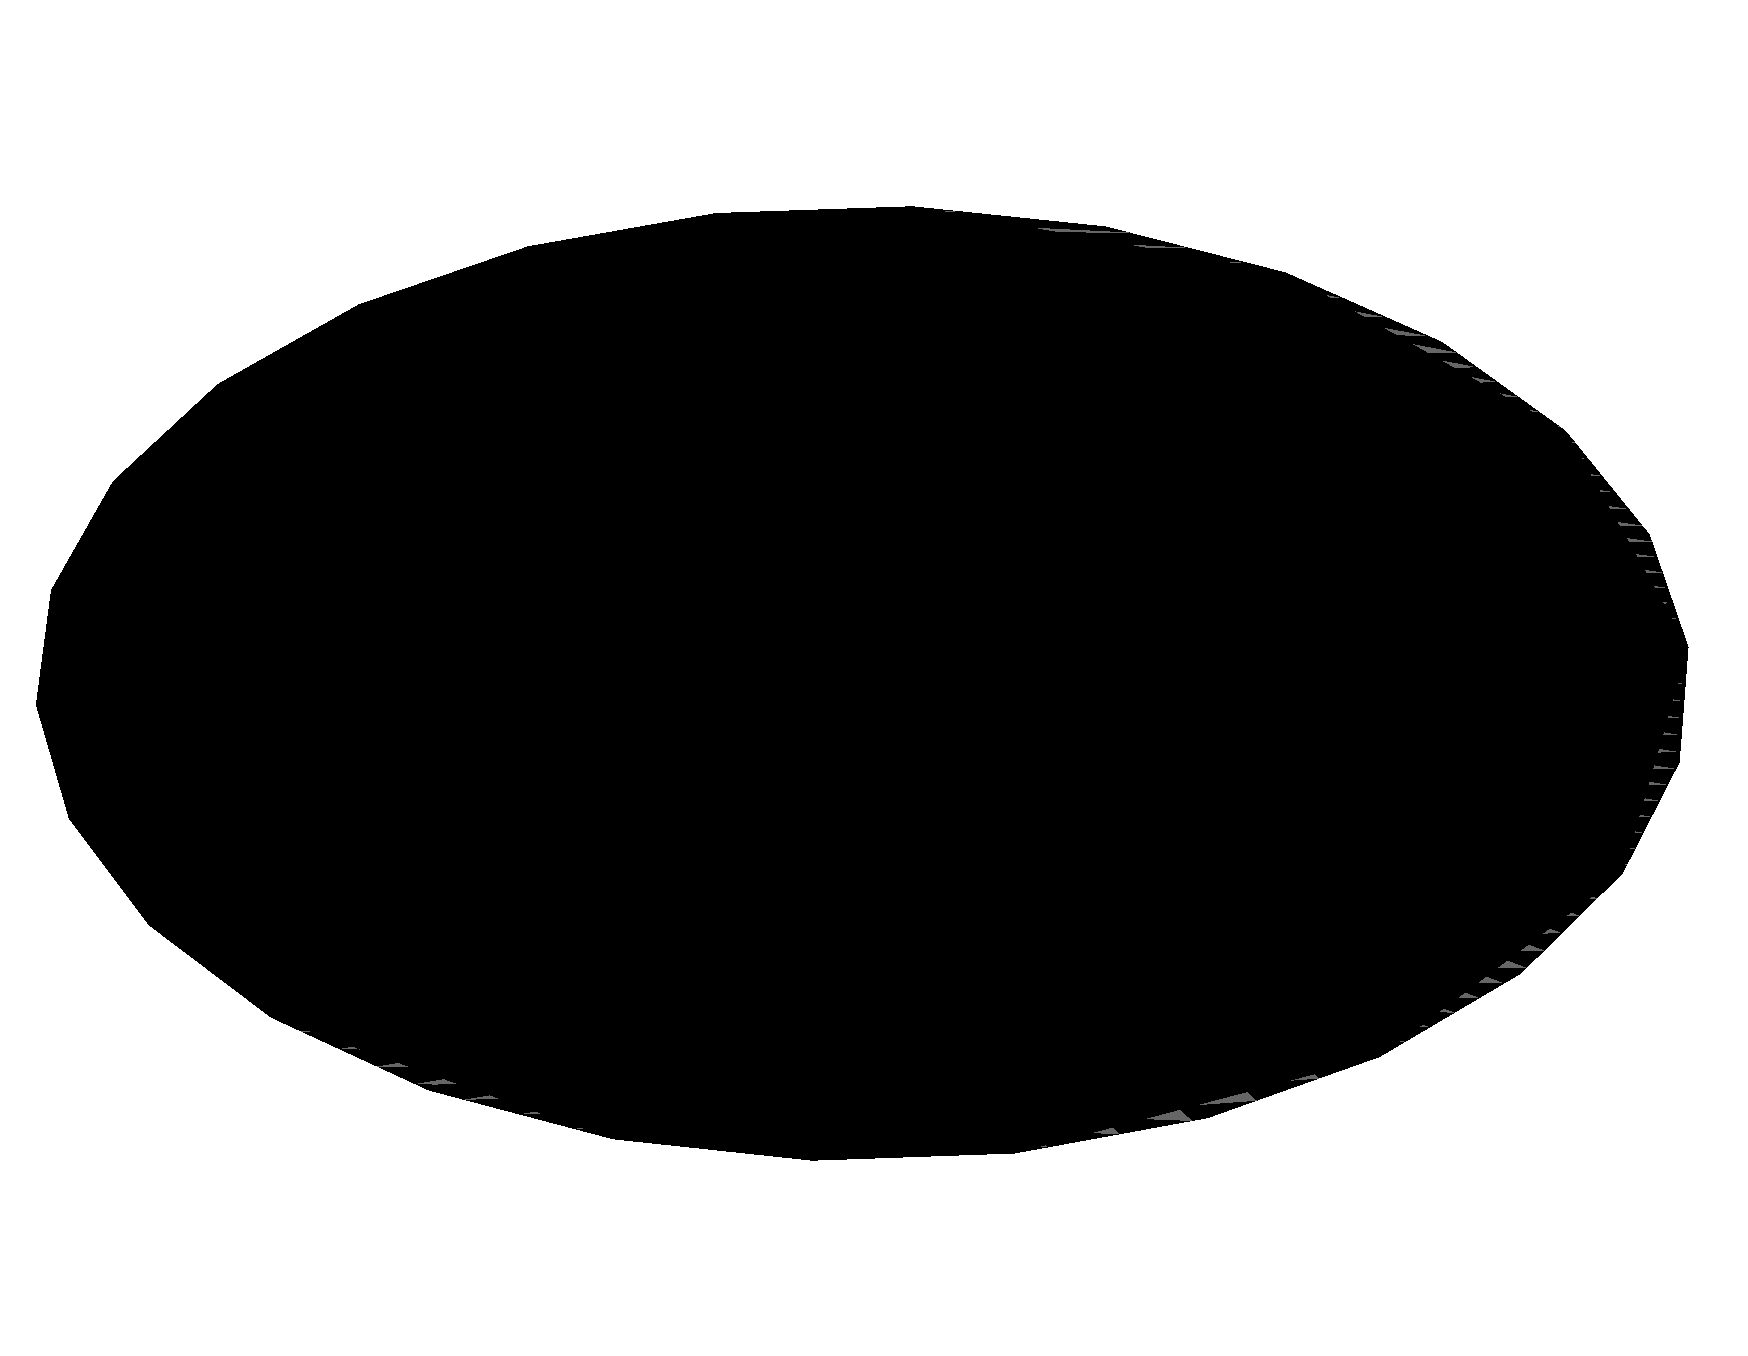
\includegraphics[width=\linewidth]{assets/images/shapes/bugold/no_height}
    \caption{\makefirstuc{WebMGA 2.0 Shape}}
    \end{subfigure}
    \begin{subfigure}{0.4\textwidth}
    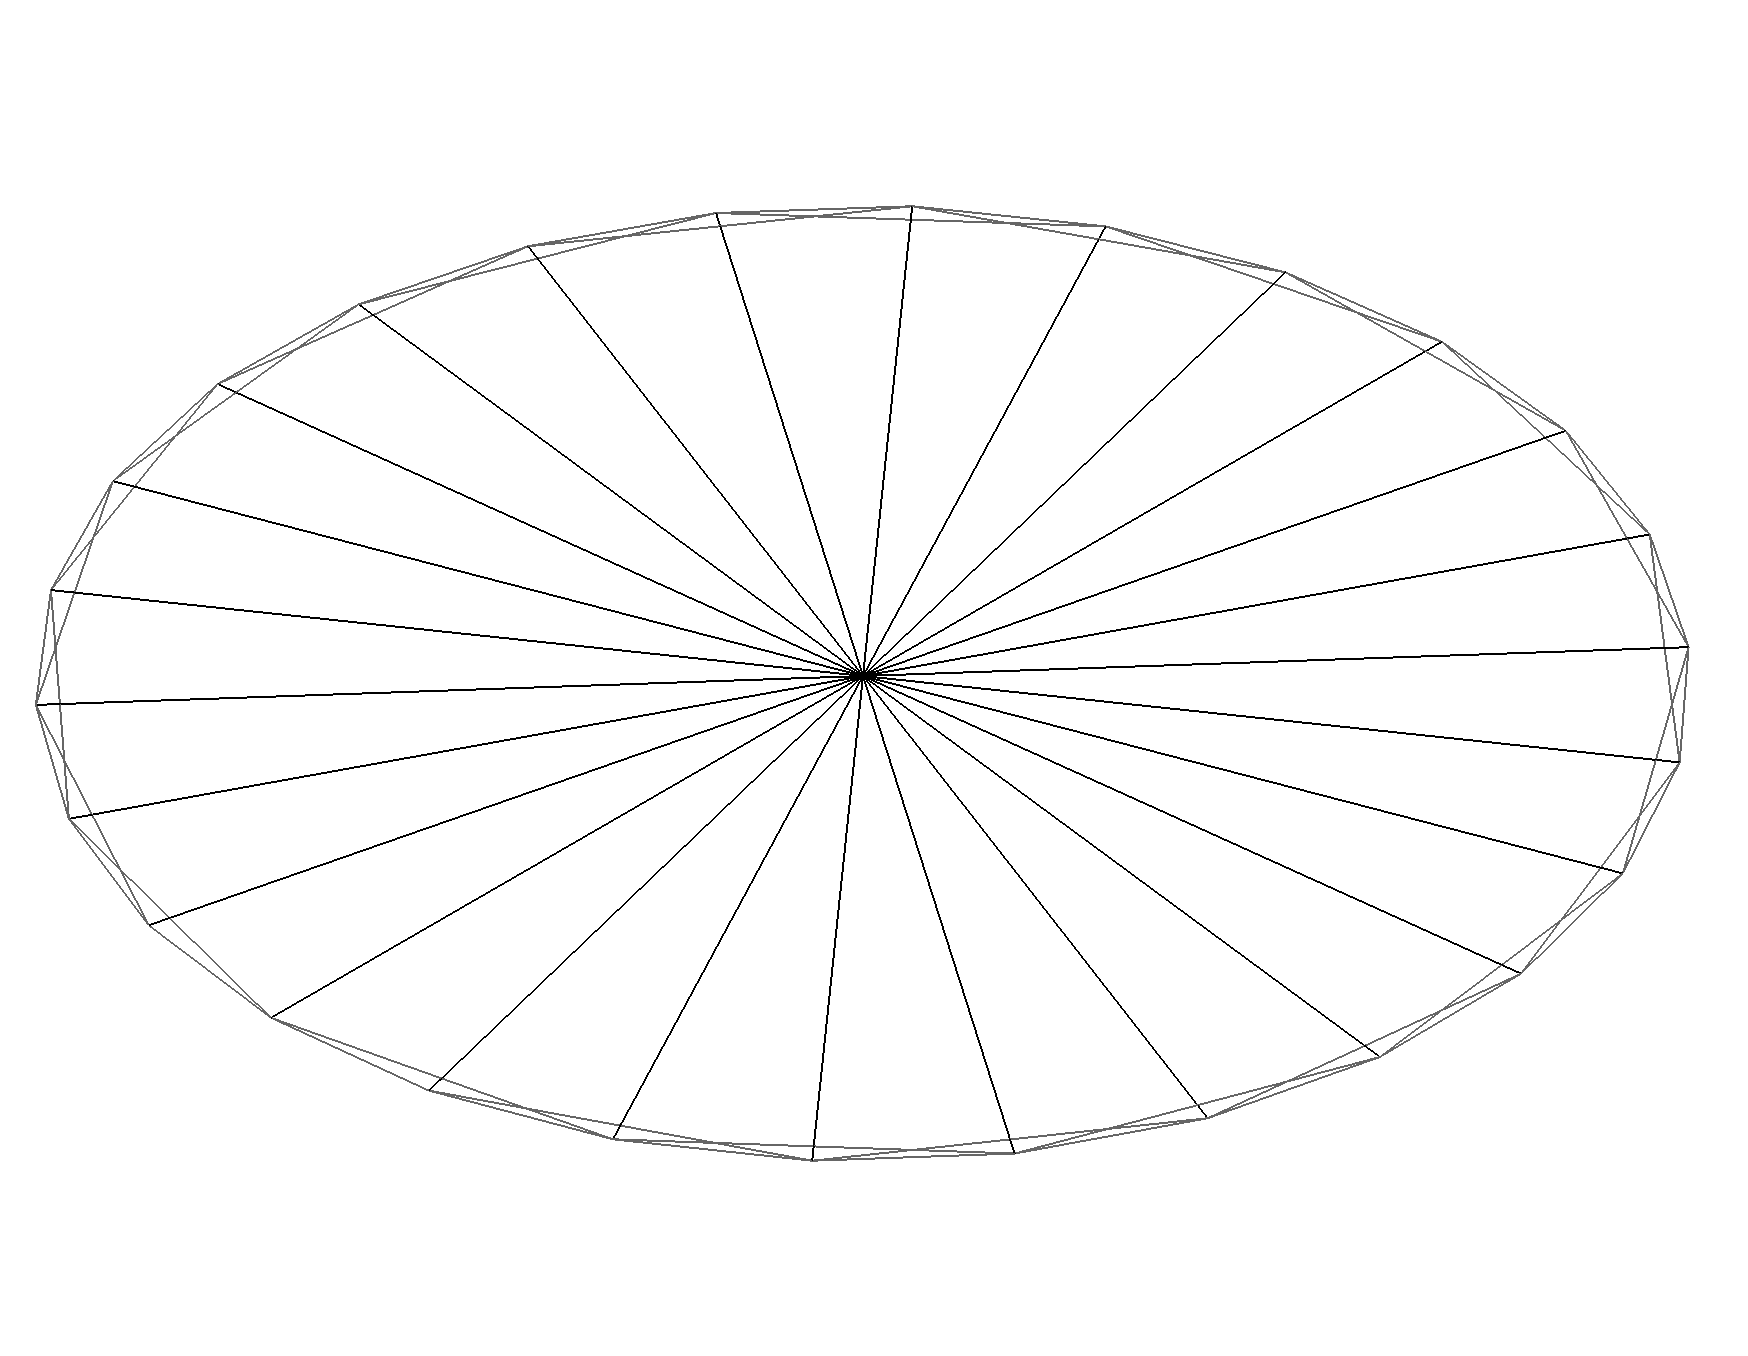
\includegraphics[width=\linewidth]{assets/images/shapes/bugold/no_height_w}
    \caption{\makefirstuc{WebMGA 2.0 Wireframe}}
    \end{subfigure}
    \begin{subfigure}{0.4\textwidth}
    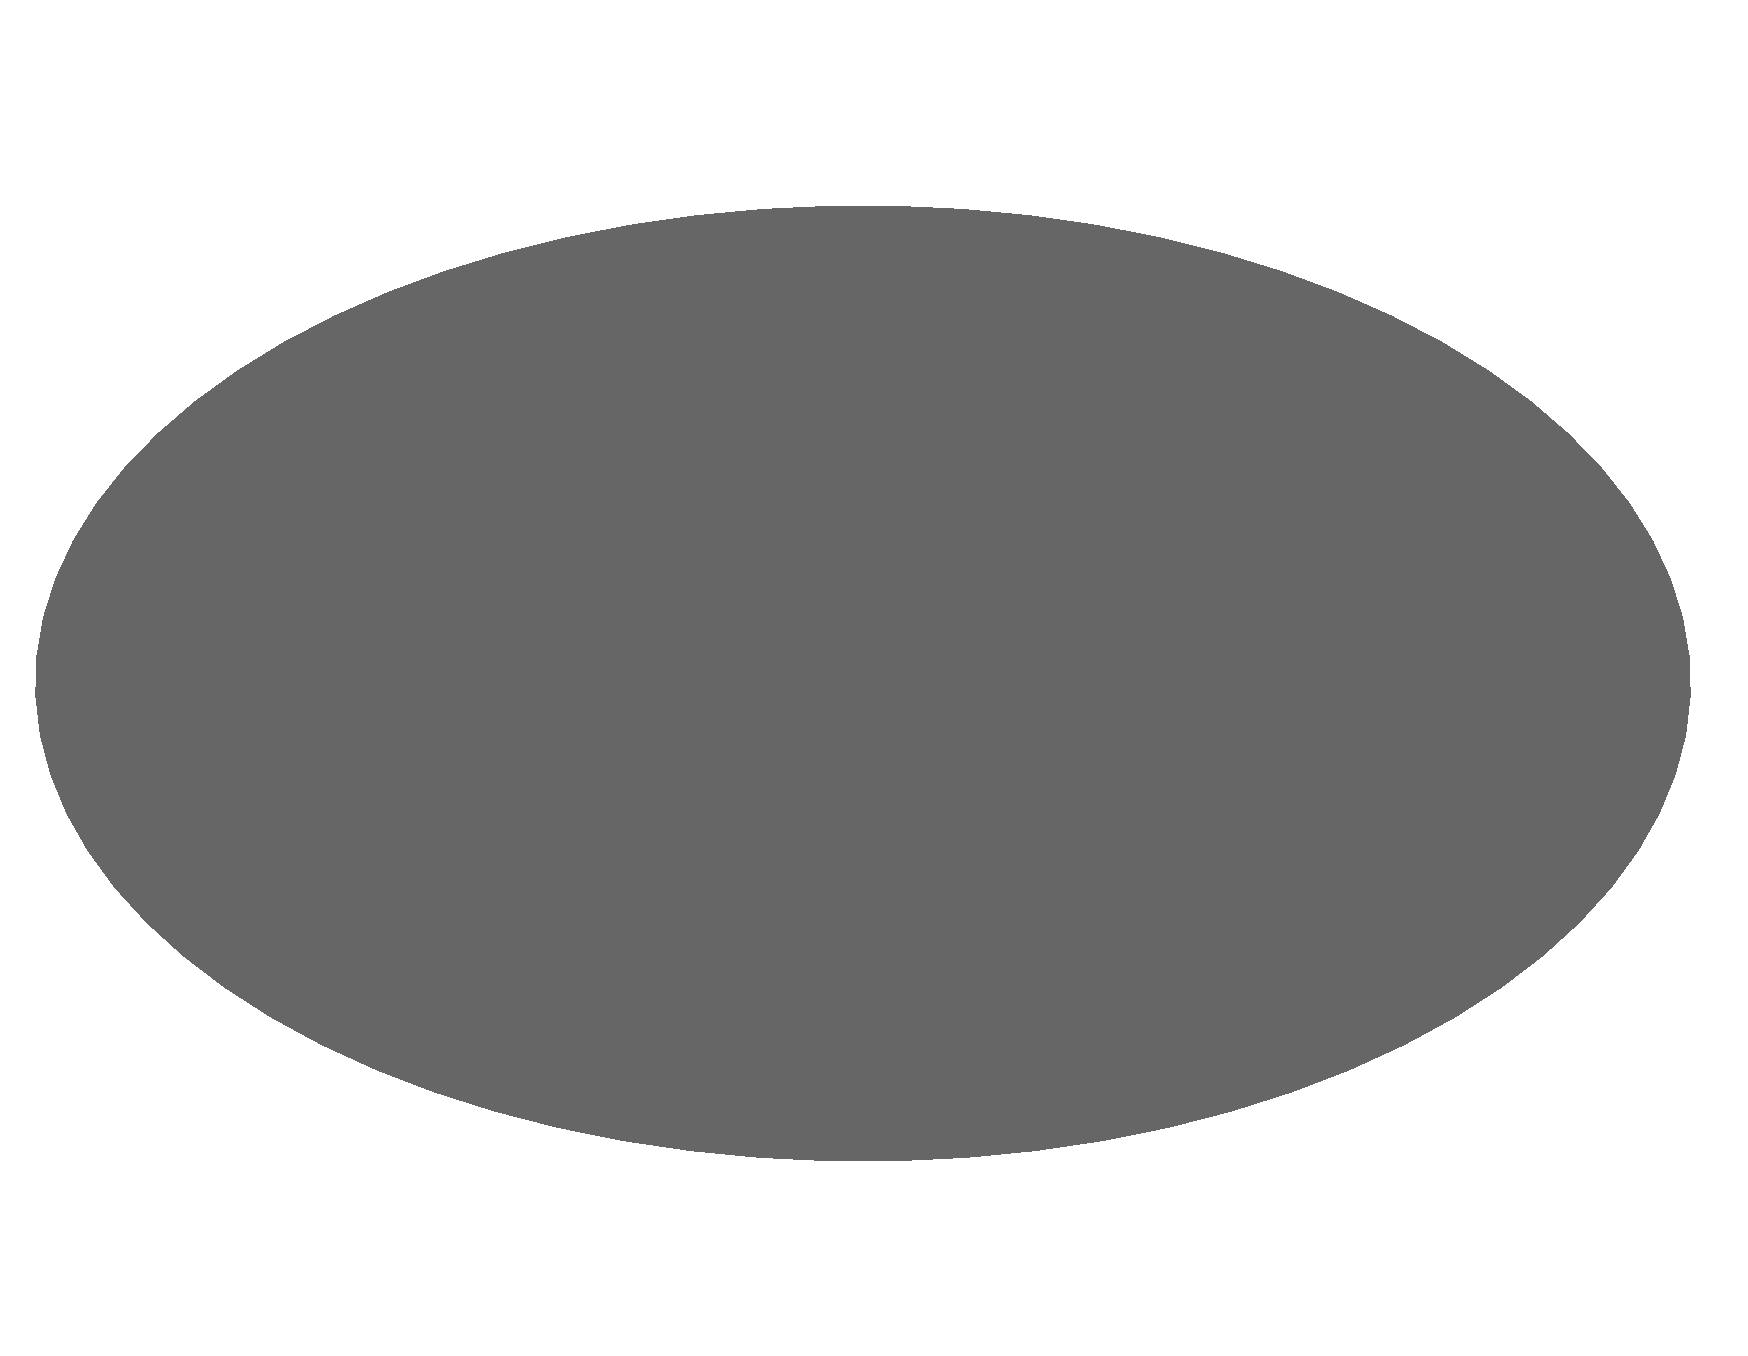
\includegraphics[width=\linewidth]{assets/images/shapes/bugnew/no_height}
    \caption{\makefirstuc{WebMGA 3.0 Shape}}
    \end{subfigure}
    \begin{subfigure}{0.4\textwidth}
    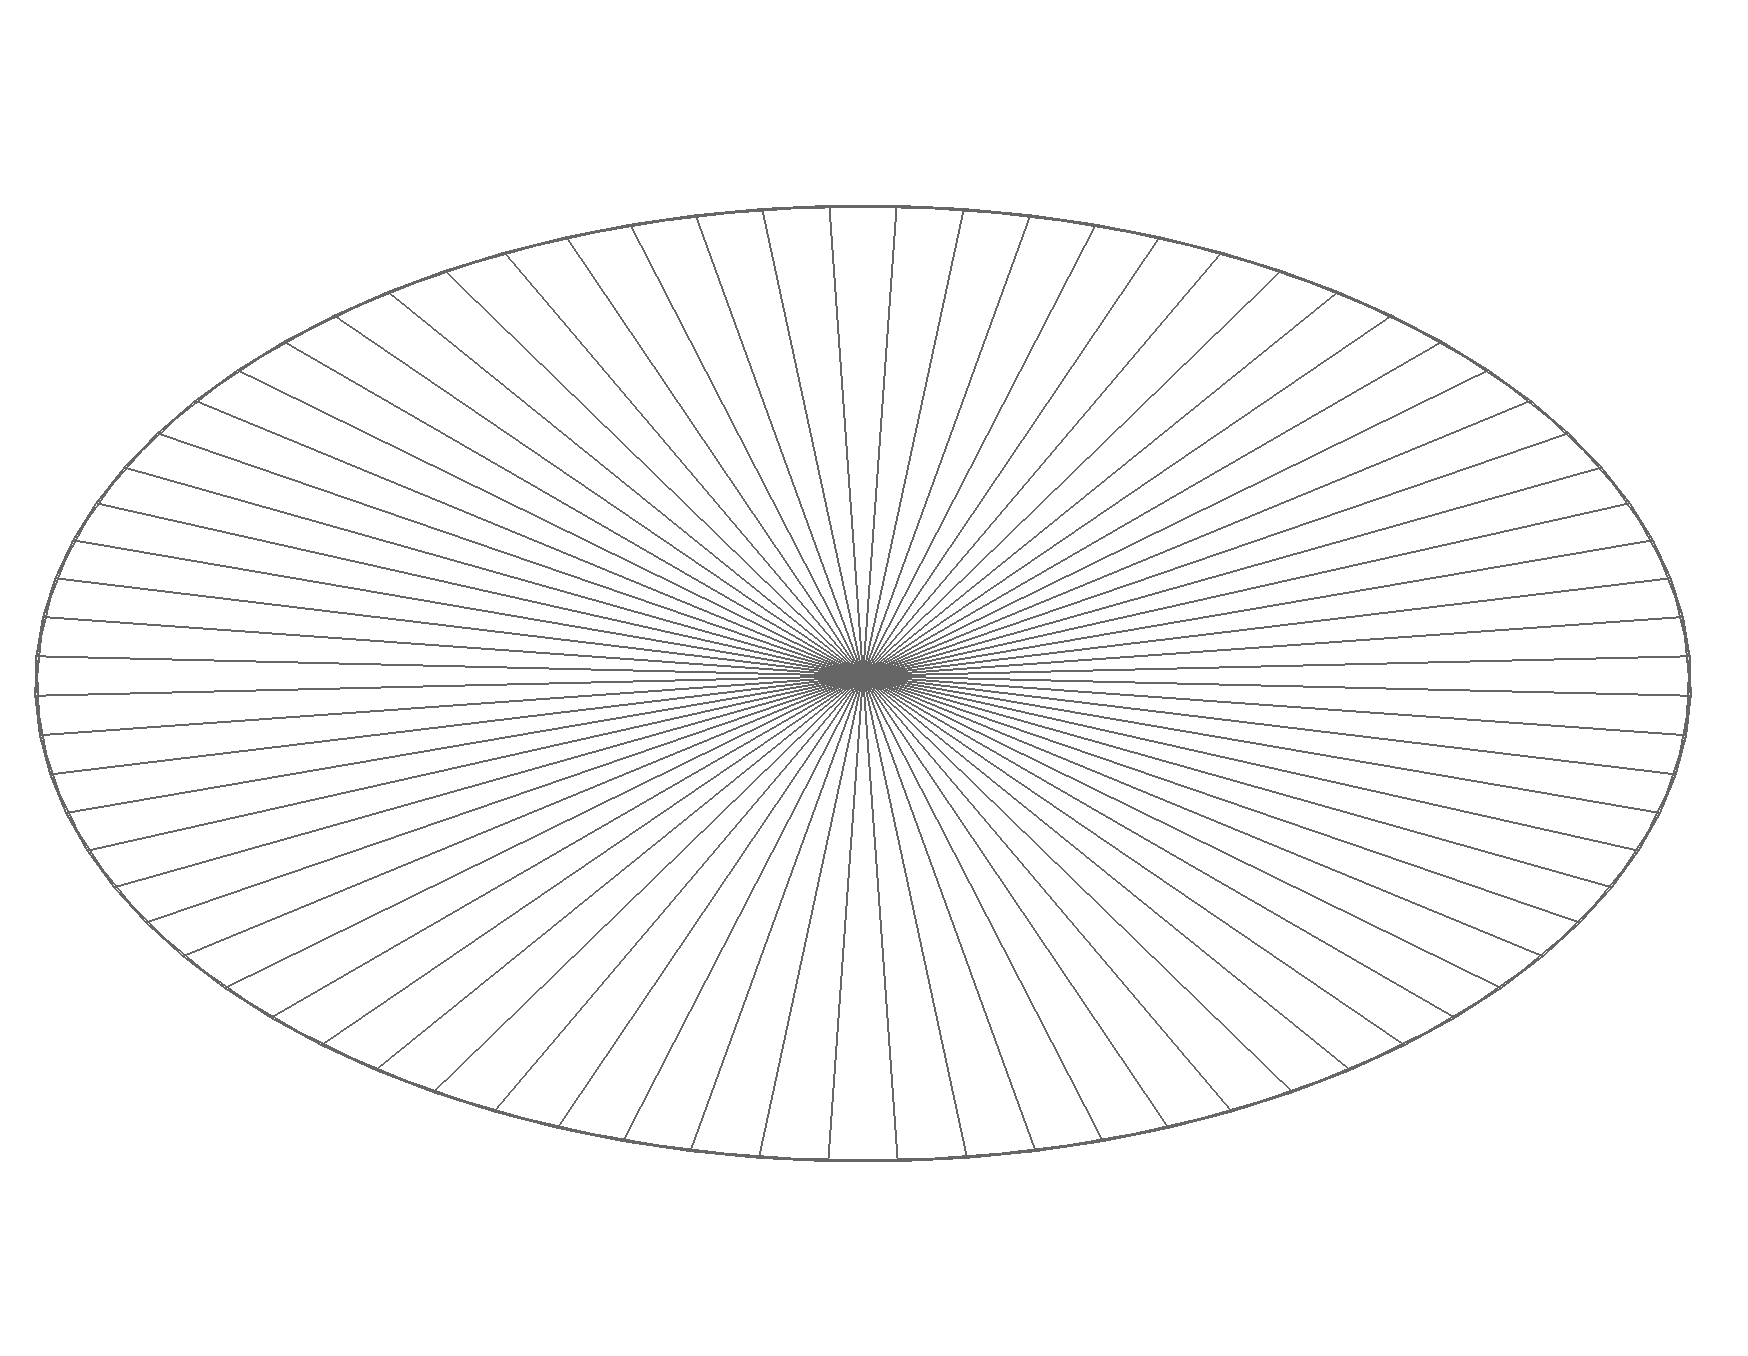
\includegraphics[width=\linewidth]{assets/images/shapes/bugnew/no_height_w}
    \caption{\makefirstuc{WebMGA 3.0 Wireframe}}
    \end{subfigure}
  \end{center}
  \caption{\makefirstuc{Buggy shape representation when double cut sphere has 0 height}}
  \label{fig:no_height_bug_old}
\end{figure}

\subsection{Improvement Goals}
\begin{itemize}
  \item Problem
    \begin{itemize}
      \item Fix
    \end{itemize}
\end{itemize}

\subsection{WebMGA 3.0 Implementation}
\subsubsection{Sphere}
Key to the new shape implementations is the implementation for the sphere (\cref{fig:sphere_shape}). The sphere mesh is generated by sampling points across the sphere's surface in such a way as to split it into a finite number of flat, triangular sub-faces as shown in \cref{fig:sphere_vertices}. This sampling is performed with the spherical coordinates system for some sphere radius $r$, azimuthal angles $\theta$, and polar angles $\phi$, converted to an equivalent Cartesian form. A point in spherical coordinate space is denoted $\mathbf{r}_{s}$, while a point in Cartesian space is denoted $\mathbf{r}_{C}$,

\begin{equation}
\mathbf{r}_\mathrm{s}=\begin{pmatrix}r\\\phi\\\theta\end{pmatrix}
\label{sphere_equation_spherical}
\end{equation}

\begin{equation}
\mathbf{r}_\mathrm{C}=\begin{pmatrix}r\sin\phi \cos\theta\\
r\sin\phi \sin\theta\\
r\cos\phi\end{pmatrix}
\label{sphere_equation_cartesian}
\end{equation}.

Any unique point on the origin centred $r$ sphere can be uniquely defined by some $(\theta,\phi)$ pair. Therefore, to evenly space points across the surface, a set of $\theta$s and $\phi$s is generated by taking $n$ (essentially a measure of mesh quality) evenly spaced values over the interval of a full circular rotation ($[0, 2\pi)$). Each unique pairing $(\phi,\gamma)$, along with $r$, is used to produce the full set of Cartesian vertices using \cref{sphere_equation_cartesian}. This method is sufficient to produce a sphere mesh as in \cref{fig:old_sphere} from WebMGA 2.0. The sampling is modified slightly for WebMGA 3.0 to produce a mesh as in \cref{fig:new_sphere} by offsetting each row such that points on one row lie half way between a pair of points on the row above since it produces a slightly more visually satisfying mesh. The code was rewritten from scratch since most other shapes result from slight modifications to the sphere generation process, and the initial WebMGA 2.0 implementation was over-complicated and proved difficult to extend.

Some optimisations can be implemented to efficiently generate a full set of vertices while sampling only $\frac{1}{4}$ of the points around the sphere's surface. This uses the fact that the origin centred sphere is symmetrical in each of the $x$, $y$, and $z$ planes. TODO FINISH THIS BIT

TODO FACE GENERATION

\begin{figure}
  \begin{center}
    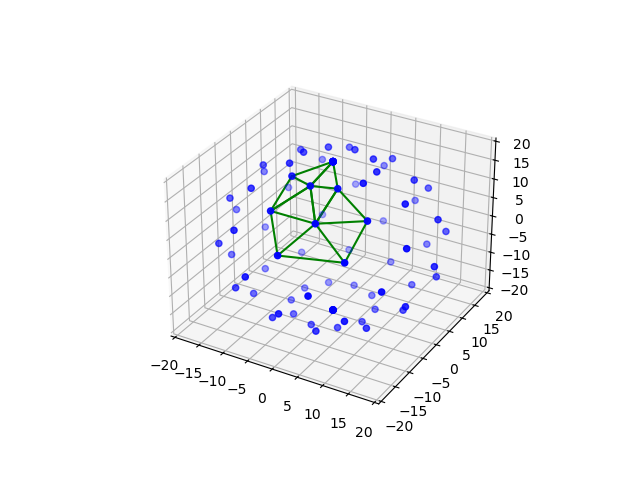
\includegraphics[width=0.5\linewidth]{assets/images/shapes/sphere_vertices}
    \caption{Example sphere vertex distribution ($9\times10$ vertical$\times$horizontal samples). Some mesh edges shown to demonstrate mesh construction from vertices.}
    \label{fig:sphere_vertices}
  \end{center}
\end{figure}

\shapefigure{sphere}{sphere}

\subsubsection{Ellipsoid}
The ellipsoid shape (\cref{fig:ellipsoid_shape}) can be represented as an origin centred sphere of radius 1 scaled in the $x$,$y$ and $z$ directions by some scalar value in each direction. This can be represented by a slightly modified form of the Cartesian sphere equation in \cref{sphere_equation_cartesian}, where $\mathbf{S}$ denotes some scaling vector,
\begin{equation}
\mathbf{r}_{e}=\begin{pmatrix}s_x r\sin\phi \cos\theta\\
s_y r\sin\phi \sin\theta\\
s_z r\cos\theta\end{pmatrix}
=\mathbf{S} \odot \mathbf{r}_\mathrm{C}
\label{ellipsoid_equation}
\end{equation}.
\shapefigure{ellipsoid}{ellipsoid}
From this formulation, it can be seen that an ellipsoid can be generated by slightly modifying the vertex sampling process for a sphere, whilst leaving the rest of the mesh building process unchanged. A sphere point can be sampled using \cref{sphere_equation_cartesian} with radius 1 and then multiplied by the scaling vector $\begin{pmatrix}s_x,s_y,s_z\end{pmatrix}^\mathsf{T}$ to give an equivalent result to \cref{ellipsoid_equation}.

In the program this is implemented by creating an ``Ellipsoid'' class as a child of the ``Sphere'' class and overriding the ``sample\_sphere()'' method. Since this implementation is so simple, the JavaScript code is provided below:

\begin{adjustbox}{width=\textwidth}
\begin{lstlisting}
//Ellipsoid mesh generator
export class Ellipsoid extends Sphere {
    //Scale factor in [x, y, z] directions
    scale: number[];

    constructor(x: number, y: number, z: number) {
        //Derive from origin centred sphere of radius 1
        super(1);
        this.scale = [x, y, z];
    }

    //Samples from ellipsoid instead of sphere
    sample_sphere(radius: number, theta: number, phi: number): number[] {
        //Multiply origin centred sphere coordinates by scale vector
        return math.dotMultiply(super.sample_sphere(radius, theta, phi), this.scale);
    }
}
\end{lstlisting}
\end{adjustbox}

\subsubsection{Spheroplatelet}
\shapefigure{spheroplatelet}{spheroplatelet}

\subsubsection{Cut Sphere}
The cut sphere shape (\cref{fig:cutsphere_shape}) is implemented simply by sampling the sphere as before but over a reduced range of $\phi$ values. Since the sphere will not be completed, an empty circular face is left which can be filled by generating an additional vertex by averaging the coordinates for each vertex on the circle's edge, splitting it into triangles. This can be observed on \cref{fig:new_cutsphere_w}.

The new range of $\phi$s can be defined as $[\arcsin\frac{c}{r}, \pi)$, where $c$ is the radius of the circle resulting from the cut and $r$ is the radius of the sphere. TODO THIS SHOULD HAVE A DIAGRAM AND BE ELABORATED ON IMPLEMENTATION
\newshapefigure{cutsphere}{cut sphere}

\subsubsection{Double Cut Sphere}
The double cut sphere shape (\cref{fig:doublecutsphere_shape}) is implemented simply by sampling the sphere as before but over a reduced range of $\phi$ values. Since the sphere will not be completed, two empty circular faces are left which can be filled by generating two additional vertices by averaging the coordinates for each vertex on the corresponding circle's edge, splitting it into triangles. This can be observed on \cref{fig:new_doublecutsphere_w}.

The new range of $\phi$s can be defined as $[\arcsin\frac{c}{r}, \pi - \arcsin\frac{c}{r})$, where $c$ is the radius of the circle resulting from the cut and $r$ is the radius of the sphere. TODO THIS SHOULD HAVE A DIAGRAM AND BE ELABORATED ON IMPLEMENTATION
\shapefigure{doublecutsphere}{double cut sphere}

\subsubsection{Cap}
\newshapefigure{cap}{cap}
The cap shape (\cref{fig:cap_shape}) is implemented simply by sampling the sphere as before but over a reduced range of $\phi$ values. Since the sphere will not be completed, an empty circular face is left which can be filled by generating an additional vertex by averaging the coordinates for each vertex on the circle's edge, splitting it into triangles. This can be observed on \cref{fig:new_cap_w}.

The new range of $\phi$s can be defined as $[0, \arcsin\frac{c}{r})$, where $c$ is the radius of the circle resulting from the cut and $r$ is the radius of the sphere. TODO THIS SHOULD HAVE A DIAGRAM AND BE ELABORATED ON IMPLEMENTATION

\subsubsection{Lens}
\paragraph{Base Lens}
\label{base_lens_para}
\paragraph{Thick Lens}
\newshapefigure{lens}{lens}

\subsubsection{Cinacchi Lens}
During development, some sample configurations requiring the lens molecule shape were provided by Giorgio Cinacchi. For these configurations, Cinacchi uses a specific lens parameterisation consisting of only a single $r$ value,
\begin{equation}
\cos\theta=1-\frac{1}{2\pi r^2}
\label{cinacchi_equations_1}
\end{equation}
\begin{equation}
\theta=\arccos\left(1-\frac{1}{2\pi r^2}\right).
\label{cinacchi_equations_2}
\end{equation}
This produces an infinitely thin lens with some aperture angle dependent on the radius. The Cinnachi lens is implemented simply as a parameterisation of the base lens in \cref{base_lens_para} where the two radii are both $r$ and angle derived from \cref{cinacchi_equations_2}.

A screenshot produced using QMGA was provided by Cinacchi to assist in visually verifying the shape produced. This is shown in \cref{fig:cinacchi_lens_provided}. A recreation was produced in QMGA as shown in \cref{fig:cinacchi_lens_qmga}, then WebMGA as shown in \cref{fig:cinacchi_lens_webmga}. This appears to verify a correct implementation.

\begin{figure}
  \begin{center}
    \begin{subfigure}{0.3\textwidth}
      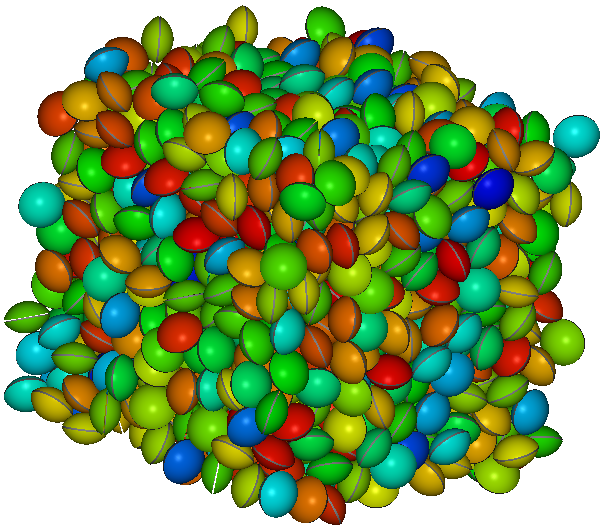
\includegraphics[width=\textwidth]{assets/images/cinacchi}
      \caption{Image by Giorgio Cinacchi.}
      \label{fig:cinacchi_lens_provided}
    \end{subfigure}
    \begin{subfigure}{0.3\textwidth}
      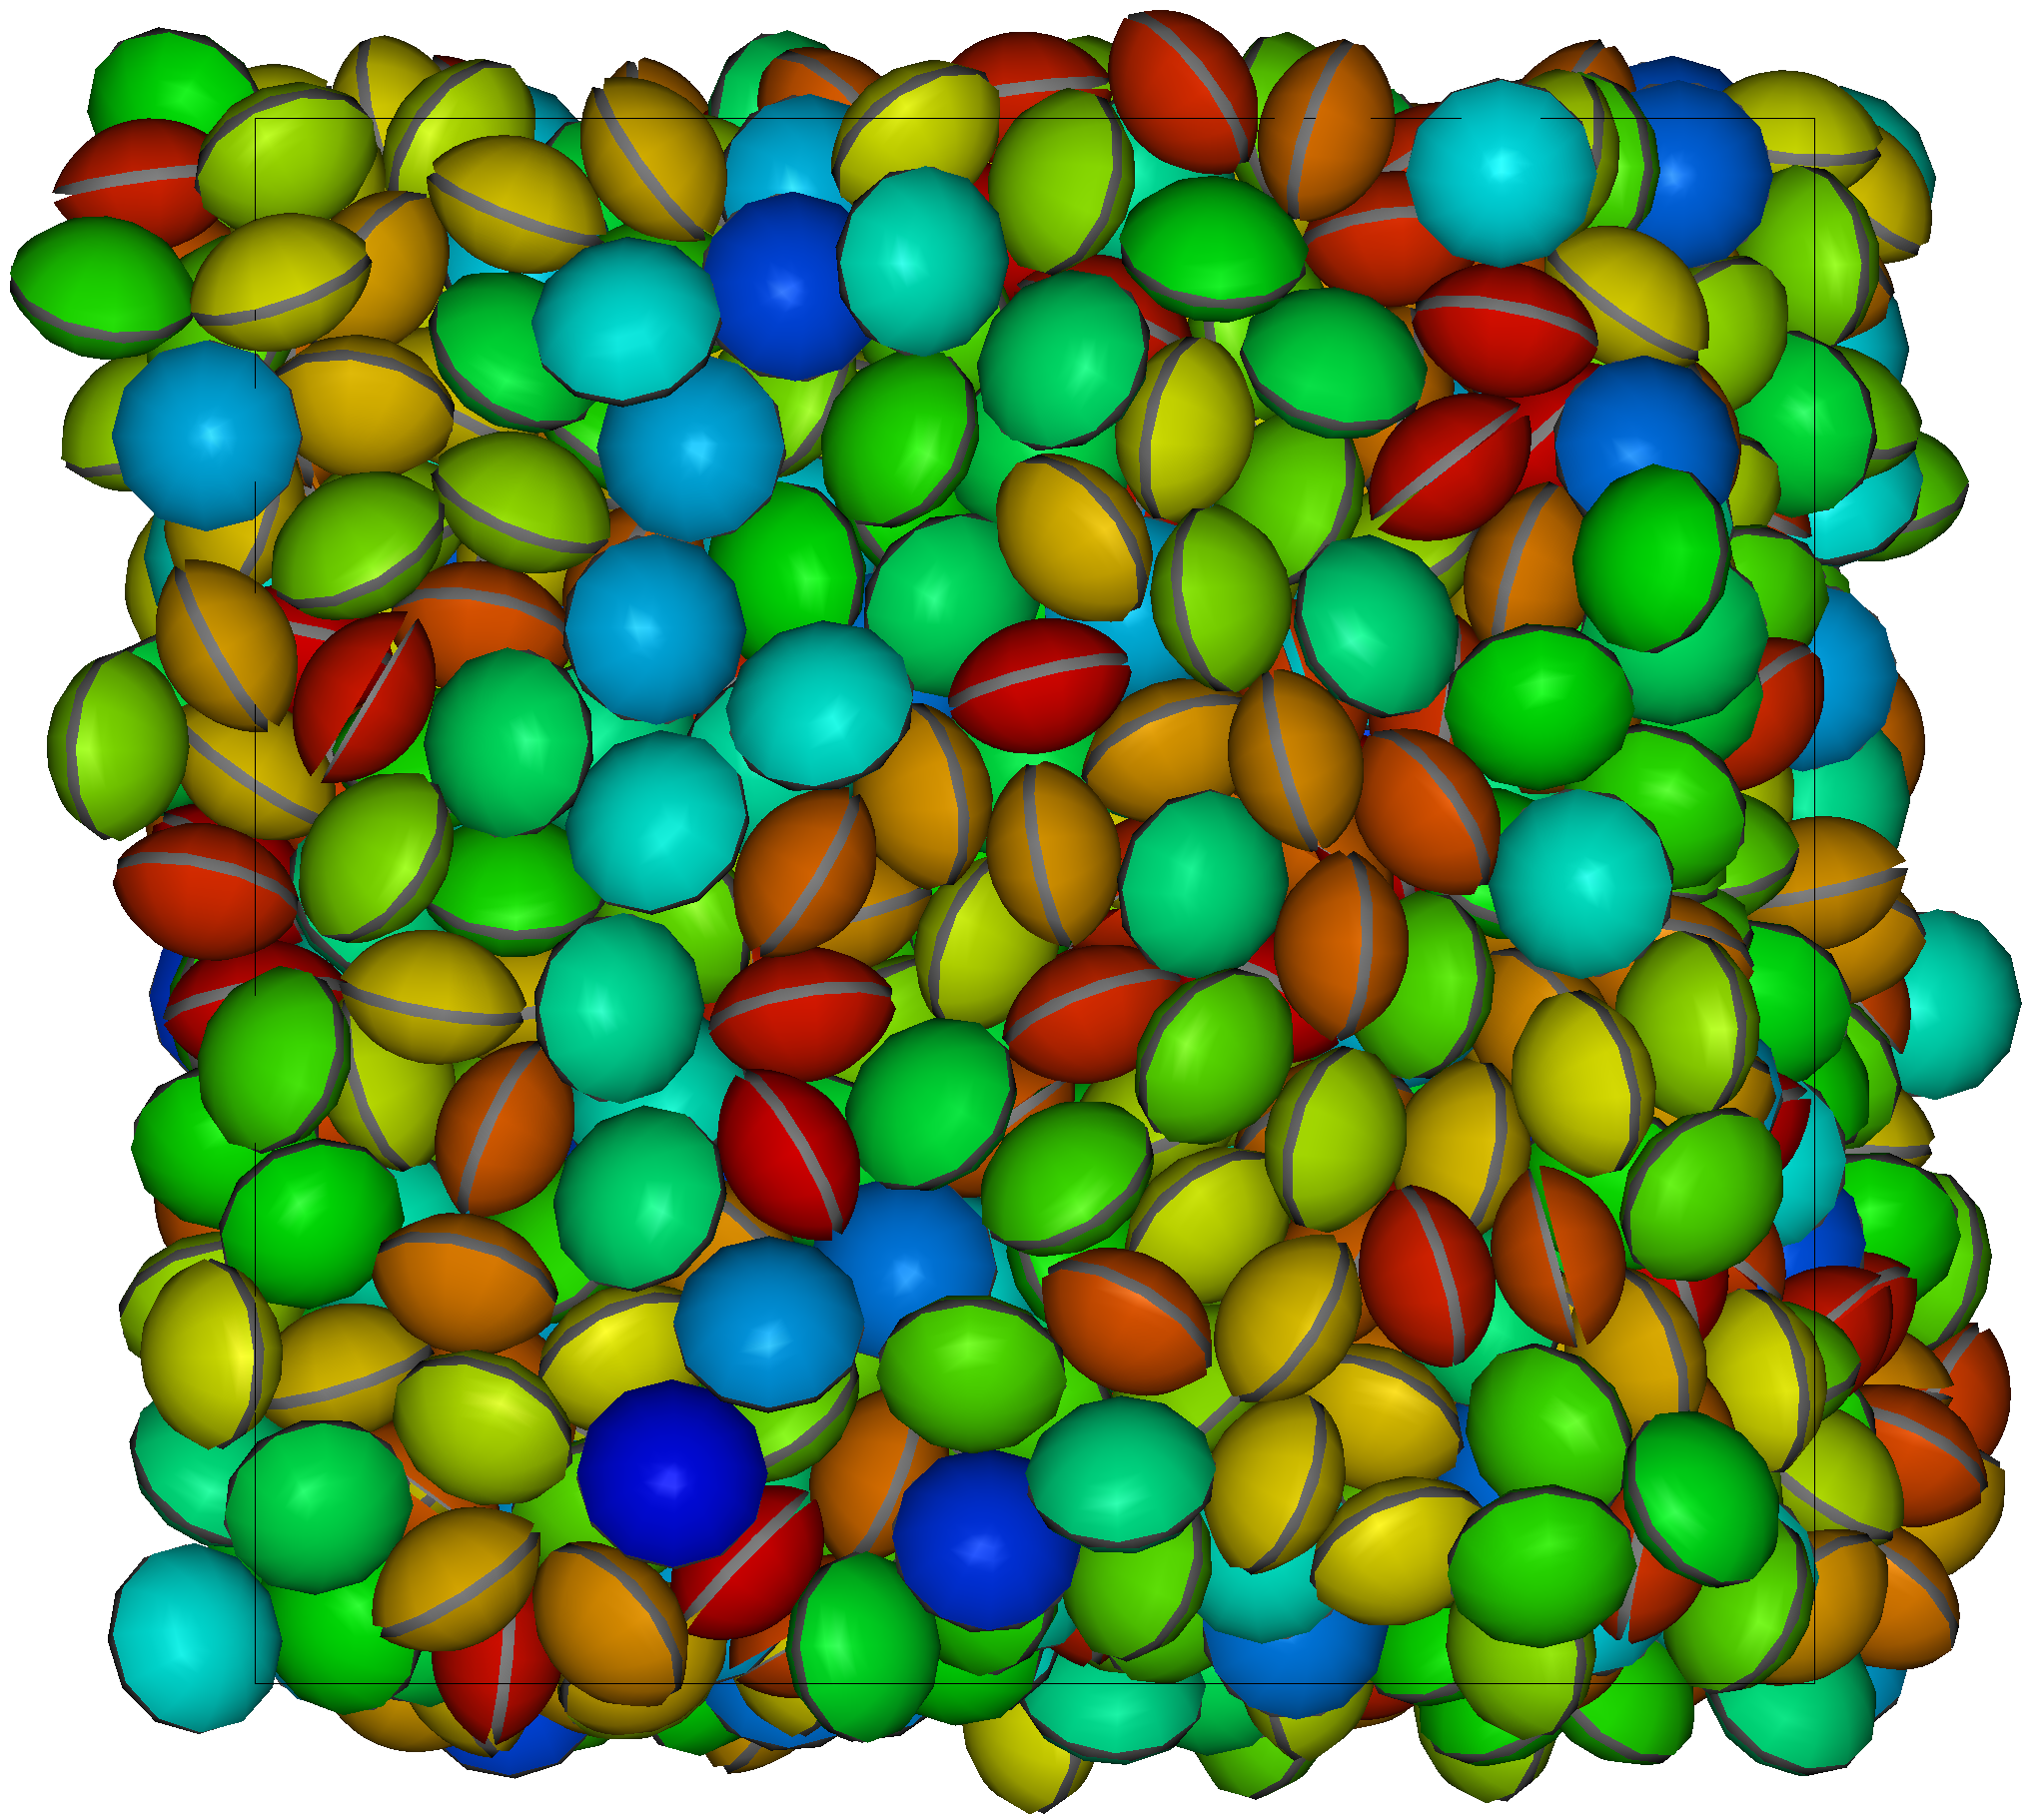
\includegraphics[width=\textwidth]{assets/images/qmga}
      \caption{Recreation with QMGA.}
      \label{fig:cinacchi_lens_qmga}
    \end{subfigure}
    \begin{subfigure}{0.3\textwidth}
      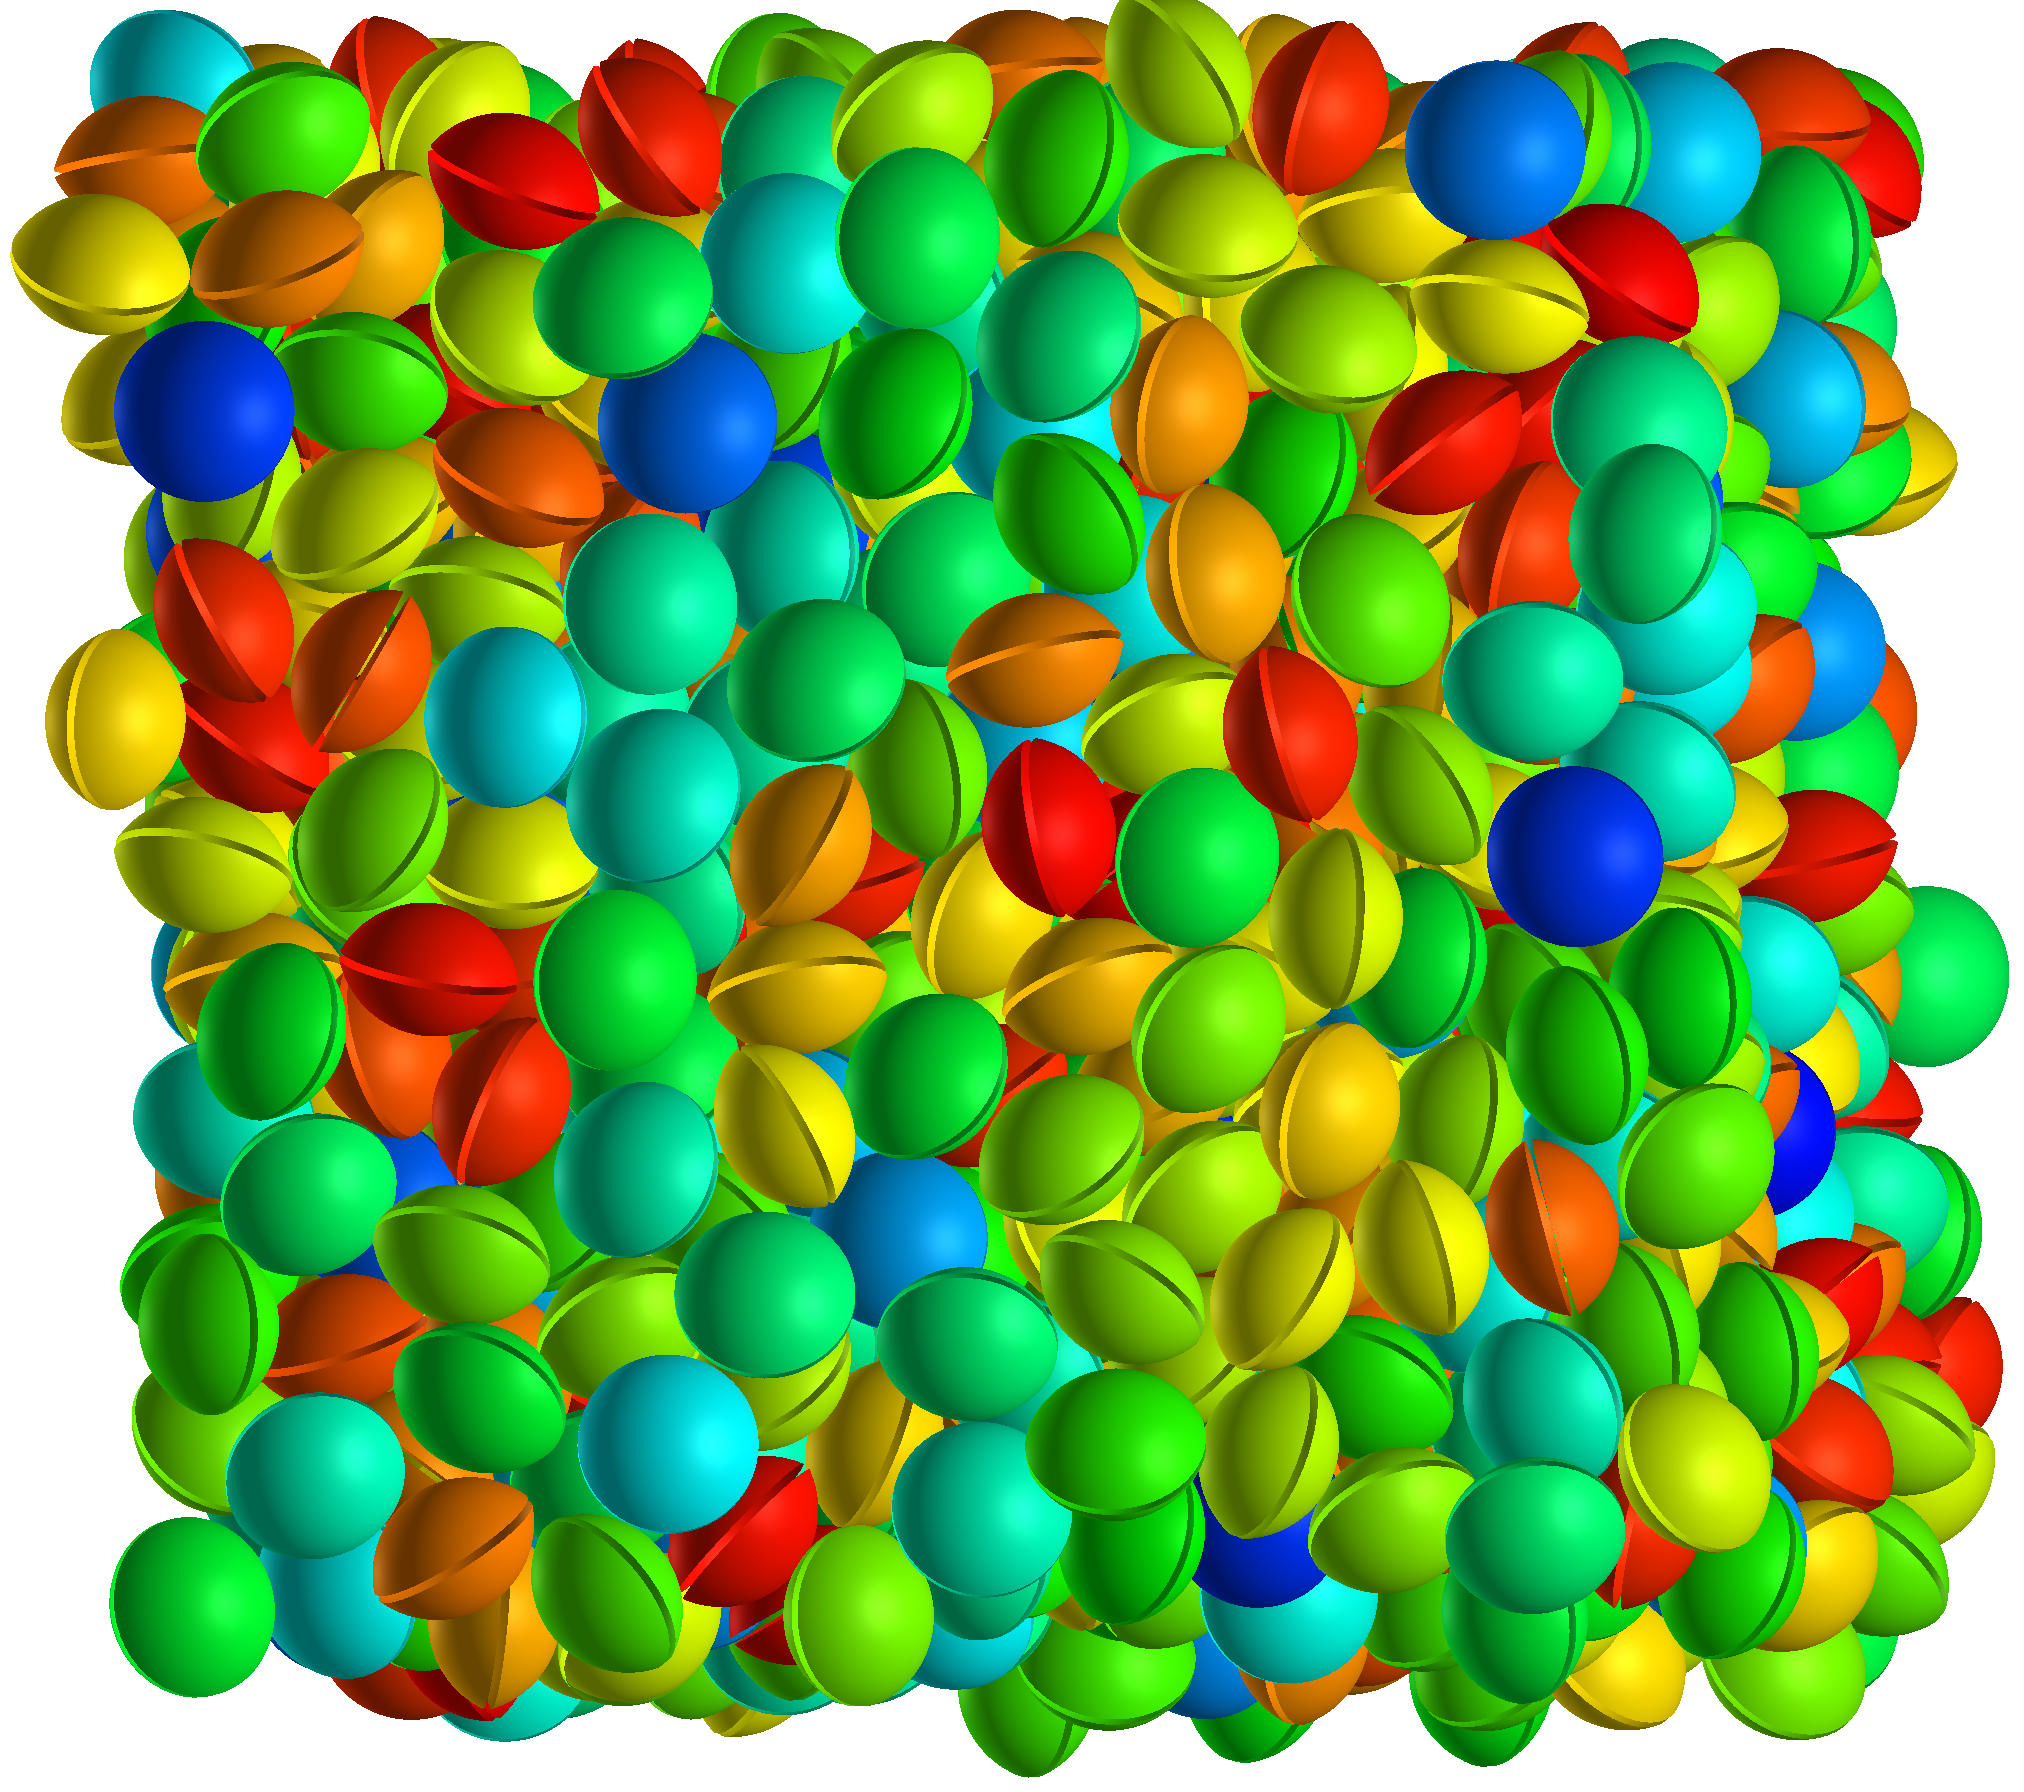
\includegraphics[width=\textwidth]{assets/images/webmga}
      \caption{Recreation with WebMGA.}
      \label{fig:cinacchi_lens_webmga}
    \end{subfigure}
  \end{center}
  \caption{Lens setup required by Giorgio Cinacchi.}
  \label{fig:cinacchi_lens}
\end{figure}

\subsubsection{Biconvex Lens}
\label{biconvex_section}
%\newshapefigure{}{}

\subsubsection{Spherocylinder}
\label{spherocylinder_section}
The spherocylinder shape (\cref{fig:spherocylinder_shape}) can be represented as an origin centred sphere of radius $r$ scaled in the $z$ directions by (half of) some length value in each $z$ direction (positive/negative). This can be represented by a slightly modified form of the Cartesian sphere equation in \cref{sphere_equation_cartesian},

\begin{equation}
\mathbf{r}_{c}=\begin{pmatrix}r\sin\phi \cos\theta\\
r\sin\phi \sin\theta\\
r\cos\theta + n\end{pmatrix}
=\mathbf{r}_{C}+\begin{pmatrix}0\\
0\\
n\end{pmatrix}
\label{spherocylinder_equation}
\end{equation}
\begin{equation}
n=\begin{cases}
  \frac{\text{length}}{2}&\text{if } r\cos\theta>0\\
  -\frac{\text{length}}{2}&\text{if } r\cos\theta<0\\
  0&\text{otherwise.}
\end{cases}
\label{spherocylinder_n_equation}
\end{equation}.
\paragraph{Initial Attempt}

From \cref{spherocylinder_equation,spherocylinder_n_equation}, it can be seen that a spherocylinder can be approximated by slightly modifying the vertex sampling process for a sphere, whilst leaving the rest of the mesh building process unchanged. A sphere point can be sampled using \cref{sphere_equation_cartesian} with radius $r$ and added to the scaling vector $\begin{pmatrix}0,0,n\end{pmatrix}^\mathsf{T}$ as defined in \cref{spherocylinder_n_equation} to give an equivalent result to \cref{spherocylinder_equation}.

In the program this was implemented by creating a ``Spherocylinder'' class as a child of the ``Sphere'' class and overriding the ``sample\_sphere()'' method. Since this implementation is so simple, the JavaScript code is provided below:

\begin{adjustbox}{width=\textwidth}
\begin{lstlisting}
//Spherocylinder mesh generator
export class Spherocylinder extends Sphere {
    //Scaling vector (either side of centre) to stretch sphere into spherocylinder ([0, 0, length / 2])
    length_scaling_vector: number[];

    constructor(radius: number, length: number) {
        //Derive from origin centred sphere of chosen radius
        super(radius);
        this.length_scaling_vector = [0, 0, length / 2];
    }

    //Samples from spherocylinder instead of sphere
    sample_sphere(radius: number, theta: number, phi: number, epsilon: number = 1e-15): number[] {
        let sphere_coordinate: number[] = super.sample_sphere(radius, theta, phi);
        //Stretch point in z direction by scale vector, matching stretch direction to sign of original vertex z
        //Unchanged if z is (approximately) 0
        if (Math.abs(sphere_coordinate[2]) < epsilon) {
        } else if (sphere_coordinate[2] > 0) {
            sphere_coordinate = math.add(sphere_coordinate, this.length_scaling_vector);
        } else if (sphere_coordinate[2] < 0) {
            sphere_coordinate = math.subtract(sphere_coordinate, this.length_scaling_vector);
        }
        return sphere_coordinate;
    }
}
\end{lstlisting}
\end{adjustbox}

\begin{figure}
  \begin{center}
    \begin{subfigure}{0.3\textwidth}
      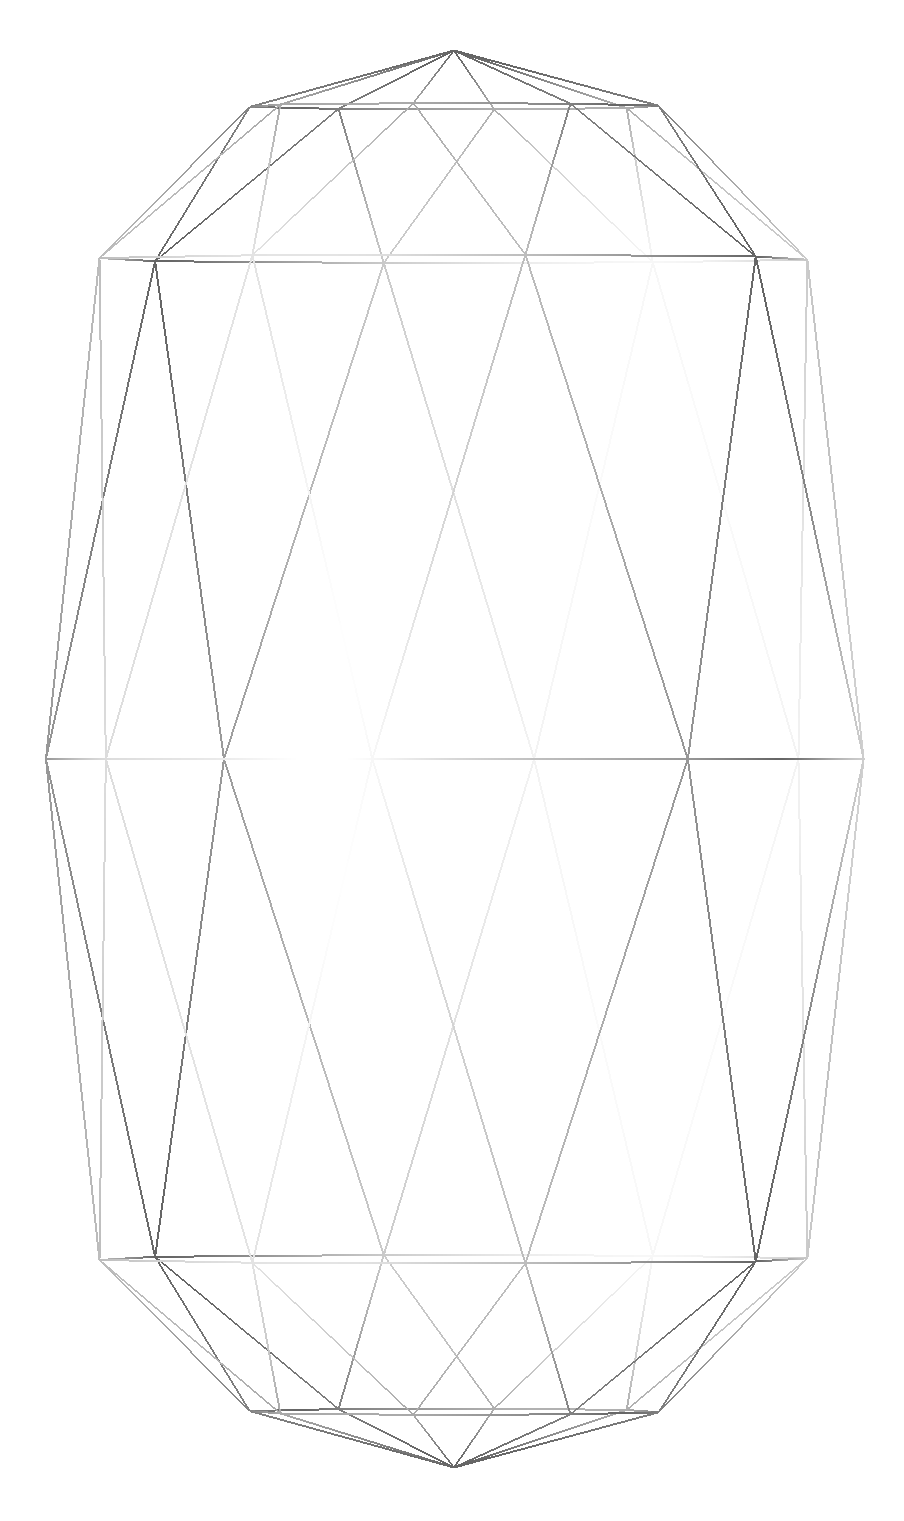
\includegraphics[width=\textwidth]{assets/images/shapes/sphero_bug/low_2}
      \caption{\makefirstuc{Low mesh density.}}
      \label{fig:sphero_bug_low_2}
    \end{subfigure}
        \begin{subfigure}{0.3\textwidth}
      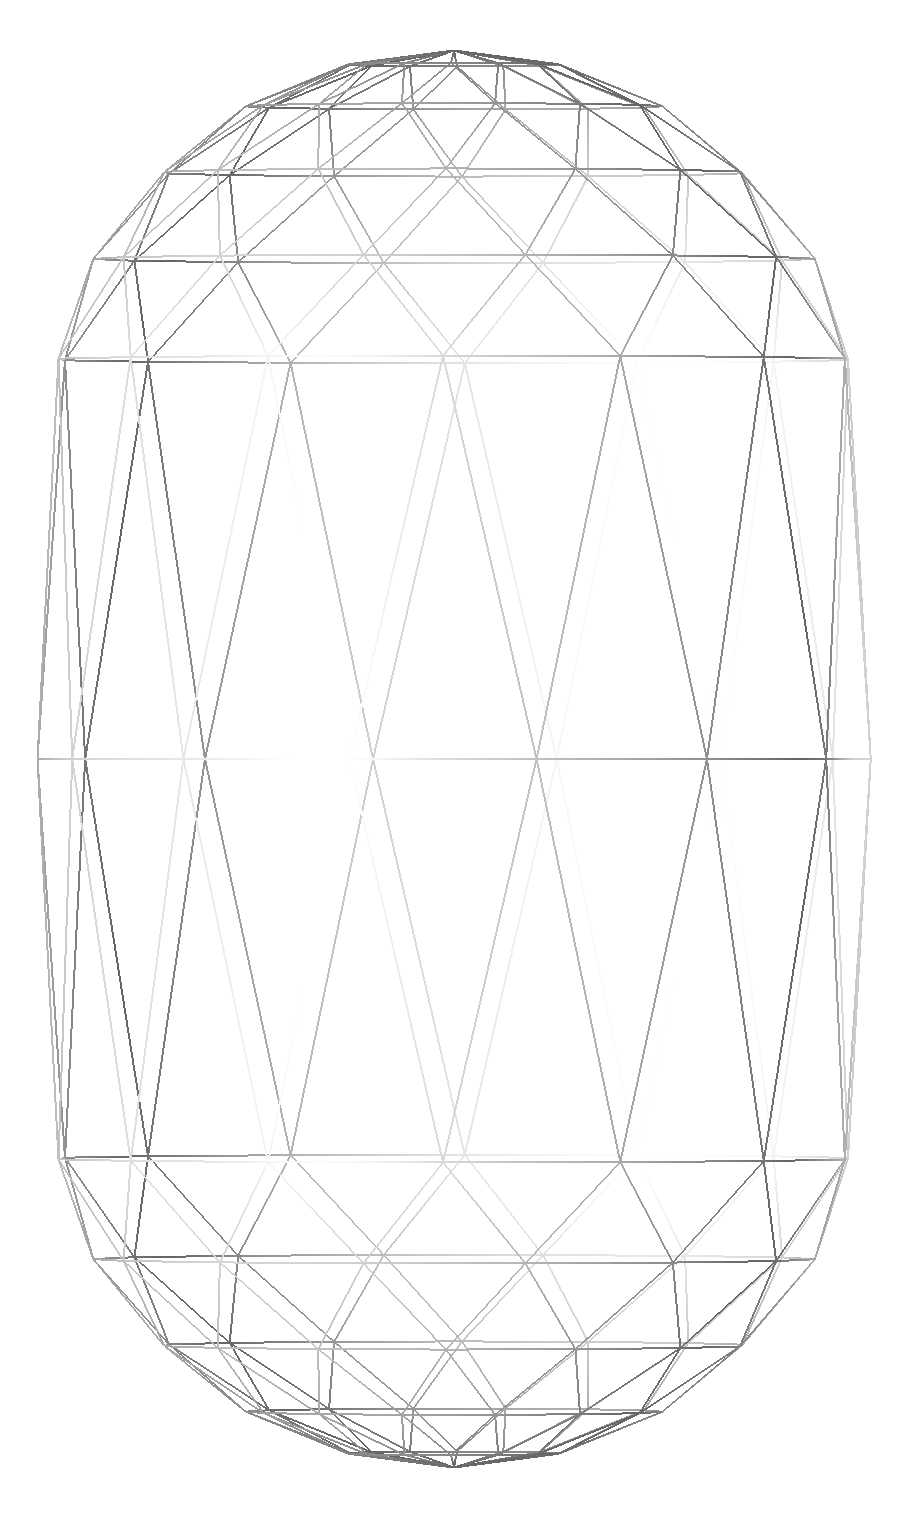
\includegraphics[width=\textwidth]{assets/images/shapes/sphero_bug/med_2}
      \caption{\makefirstuc{Medium mesh density.}}
      \label{fig:sphero_bug_med_2}
    \end{subfigure}
        \begin{subfigure}{0.3\textwidth}
      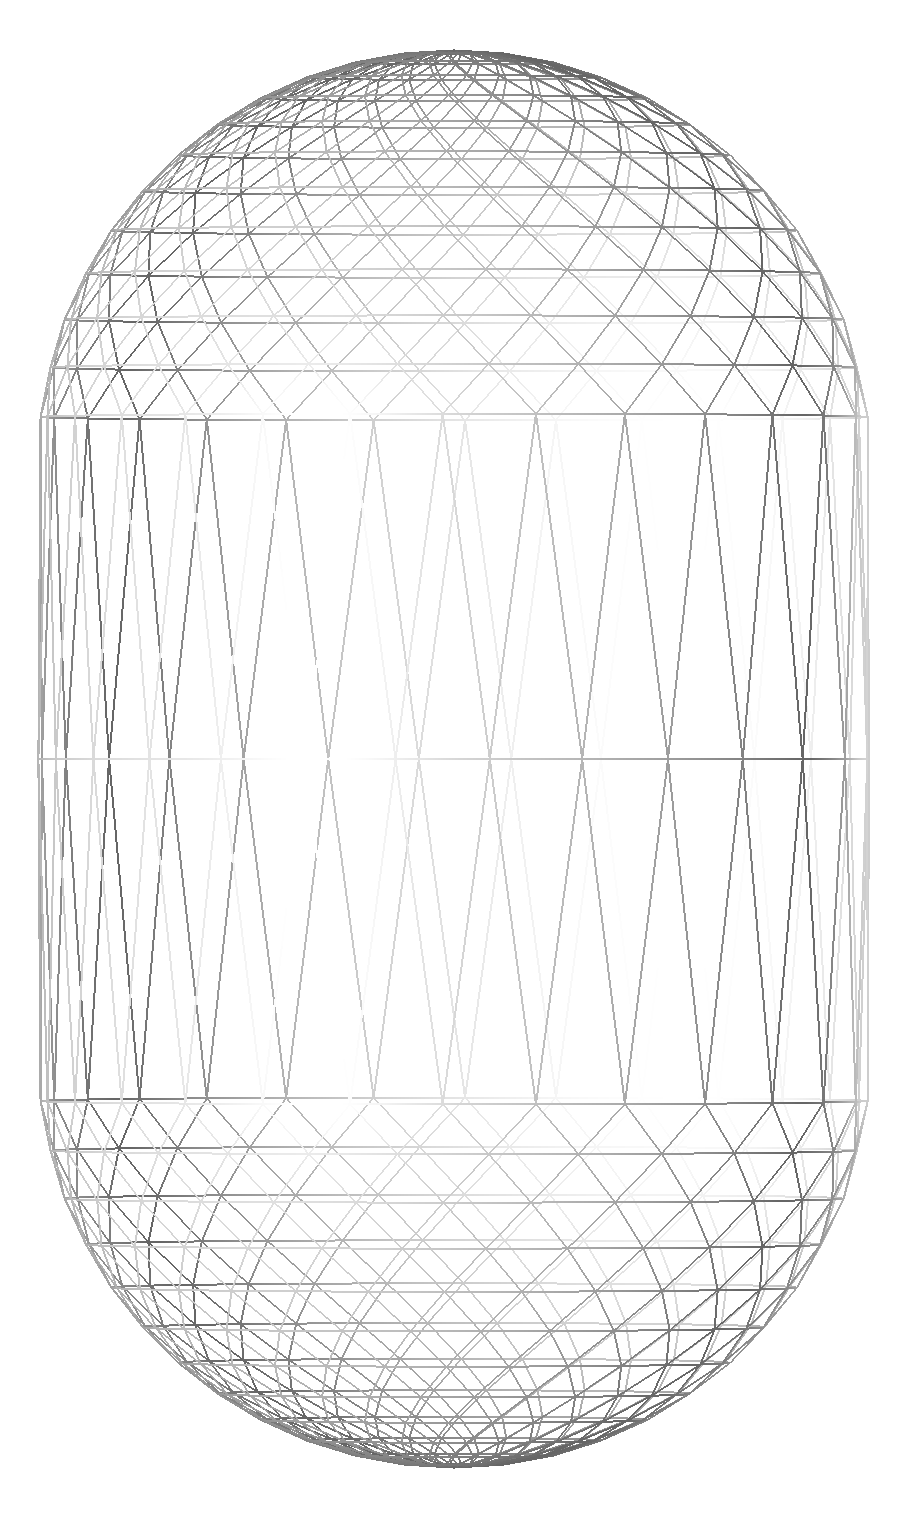
\includegraphics[width=\textwidth]{assets/images/shapes/sphero_bug/high_2}
      \caption{\makefirstuc{High mesh density.}}
      \label{fig:sphero_bug_high_2}
    \end{subfigure}
  \end{center}
  \caption{Initial spherocylinder implementation. Visible tapering can be observed, particularly with low mesh density.}
  \label{fig:sphero_bug}
\end{figure}
Unfortunately, this process produced visually unsatisfying results with the sides of the spherocylinder visibly tapering, particularly with low detail meshes. This can be seen in \cref{fig:sphero_bug}. After producing the biconvex lens (\cref{biconvex_section}), an alternate, much simpler solution became apparent which avoided this issue.
\paragraph{Second Attempt}

A spherocylinder can also be considered a special case of the biconvex lens. A biconvex lens with no separation and aperture angle $\frac{\pi}{2}$ produces a sphere with the given radius $r$. Increasing the separation parameter causes the two hemispheres to move apart such that a spherocylinder is produced. The spherocylinder can therefore simply be considered a special case of the biconvex lens with aperture angle $\frac{\pi}{2}$, and can be implemented entirely through class inheritance as shown:
\begin{lstlisting}
//Spherocylinder mesh generator
export class Spherocylinder extends BiconvexLens {
    constructor(radius: number, length: number) {
        super(radius, Math.PI / 2, length);
    }
}
\end{lstlisting}
This produced the result shown in \cref{fig:spherocylinder_shape}.
\shapefigure{spherocylinder}{spherocylinder}

\subsection{WebMGA 3.0 Bugs}
TODO
